\documentclass[UTF-8]{article}
\usepackage{amsmath}
\usepackage{amssymb}
\usepackage{float}
\usepackage{graphicx}
\usepackage{epstopdf}
\usepackage{inputenc}
\usepackage{geometry}
\usepackage{pgfplots} 
\usepackage{listings}
\usepackage{color}
\usepackage{hyperref}
\usepackage{enumerate}
\geometry{left=2.5cm,right=2.5cm,top=2.5cm,bottom=2.5cm}

\definecolor{codegreen}{rgb}{0,0.6,0}
\definecolor{codegray}{rgb}{0.5,0.5,0.5}
\definecolor{codepurple}{rgb}{0.58,0,0.82}
\definecolor{backcolour}{rgb}{0.9,0.9,0.92}

\lstdefinestyle{mystyle}{
	backgroundcolor=\color{backcolour},   
	commentstyle=\color{codegreen},
	keywordstyle=\color{blue},
	numberstyle=\tiny\color{codegray},
	stringstyle=\color{codepurple},
	basicstyle=\ttfamily\footnotesize,
	breakatwhitespace=false,         
	breaklines=true,                 
	captionpos=b,                    
	keepspaces=true,                 
	numbers=left,                    
	numbersep=5pt,                  
	showspaces=false,                
	showstringspaces=false,
	showtabs=false,                  
	tabsize=2
}

\lstset{style=mystyle}


\title{Computer Vision 2023 \\
	\large Assignment 3} %exchange for assignment number

\author{Sebastian Bergner}
\begin{document}
	
	\maketitle
	
	\section*{Task 1}
	(5 points) Make a very short video with your camera.
	\begin{enumerate}[a.]
		\item Compute  and  show  the  disparity  map  using  OpenCV  for  two  nearby 
		frames. \href{https://docs.opencv.org/4.x/dd/d53/tutorial_py_depthmap.html}{OpenCV disparity map tutorial.}
		\\The two near frames are one arbitrary image and the next one so $i$ and $i+1$.
		\begin{figure}[H]
			\centering
			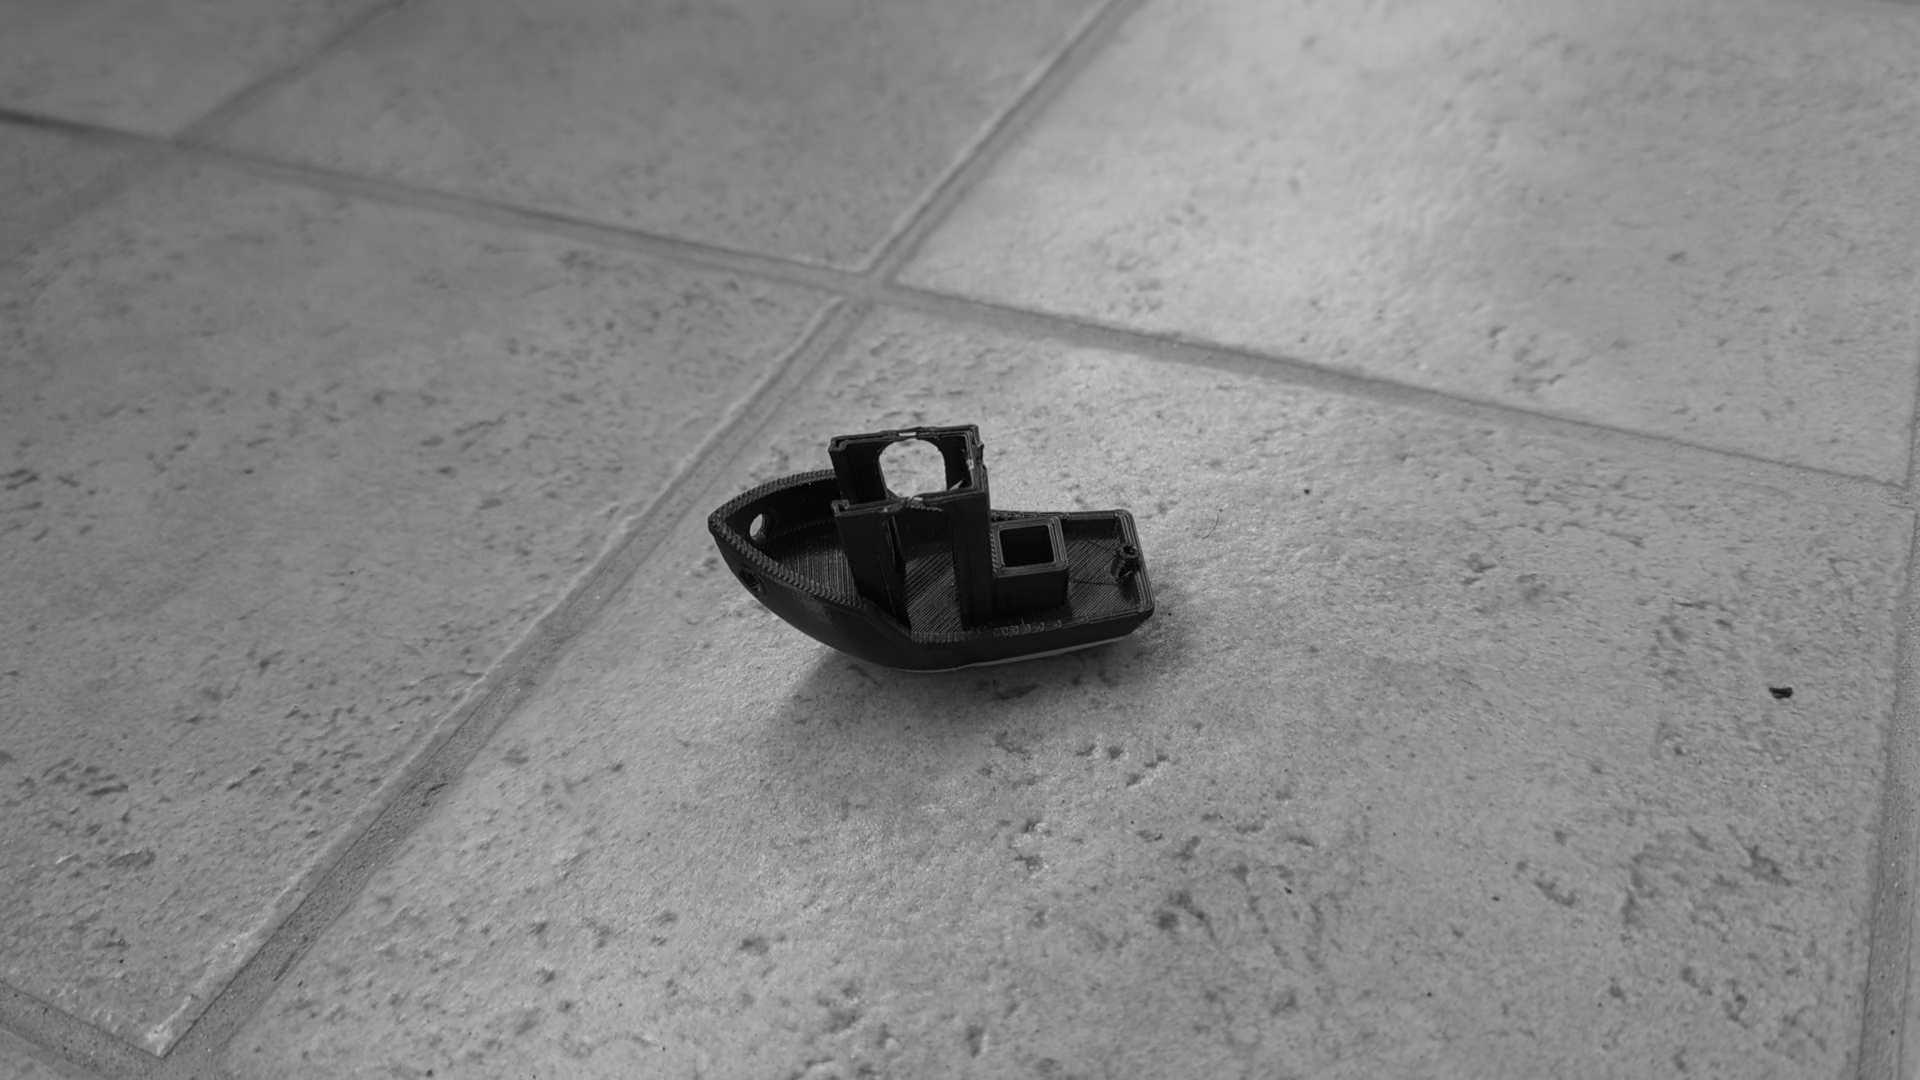
\includegraphics[width=0.7\linewidth]{images/exercise1/videooutimg1}
			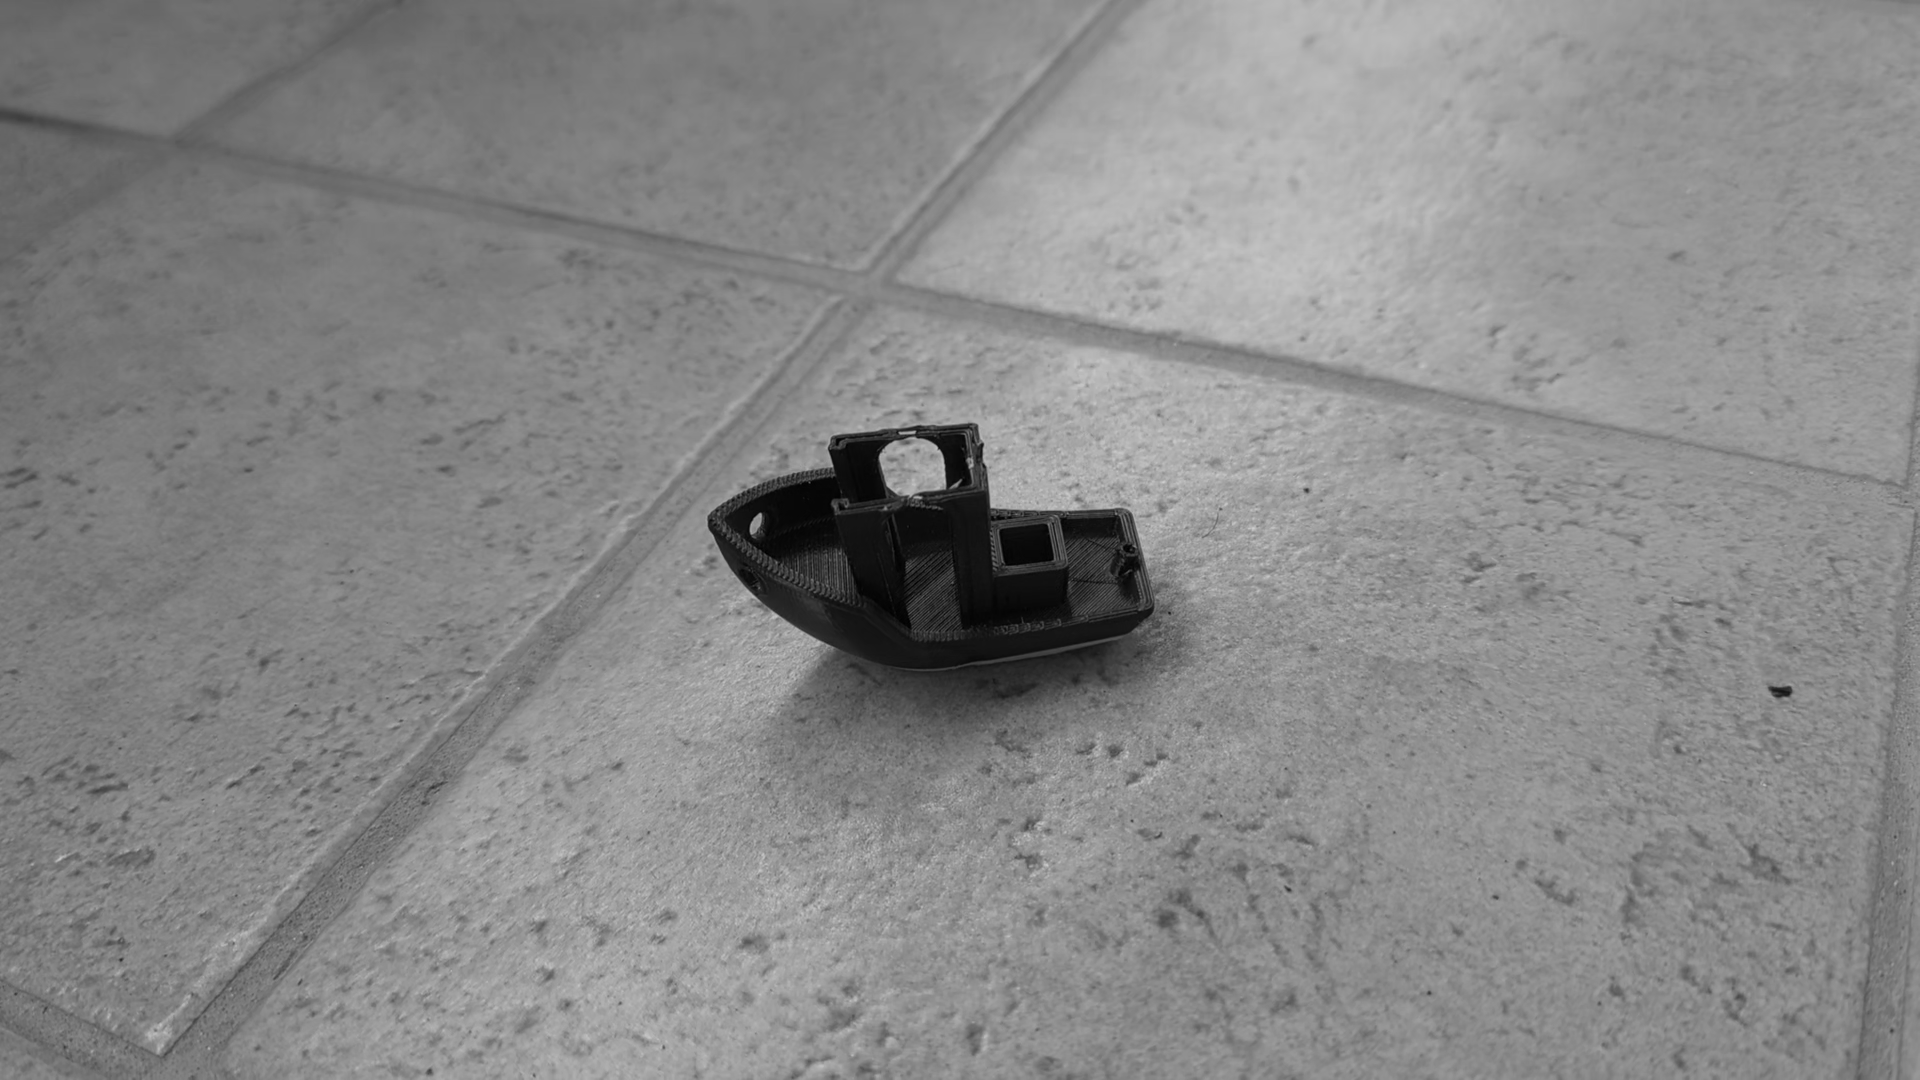
\includegraphics[width=0.7\linewidth]{images/exercise1/videooutimg2}
			\caption{Near input images.}
			\label{fig:videooutimg1}
		\end{figure}
		And the resulting disparity map.
		\begin{figure}[H]
			\centering
			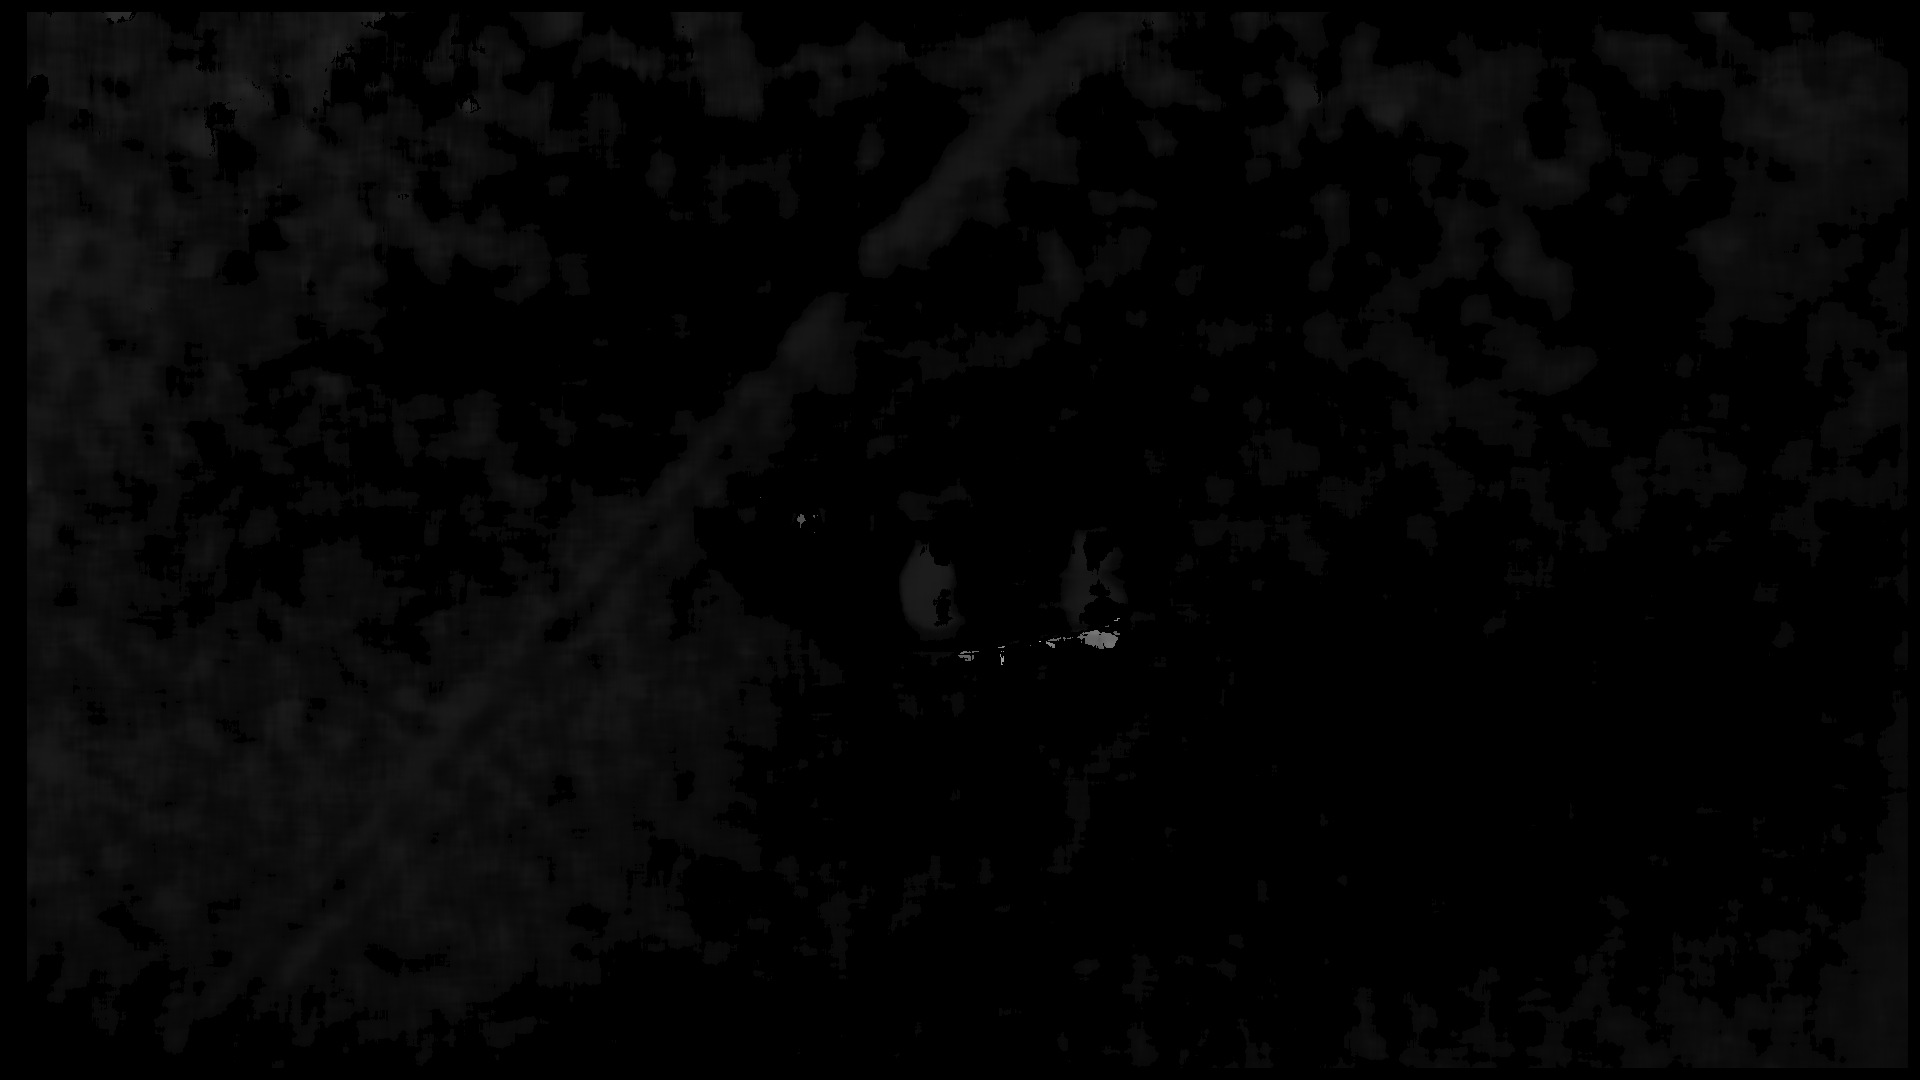
\includegraphics[width=0.7\linewidth]{images/exercise1/videodisparity_near.png}
			\caption{Disparity map using near frames.}
			\label{fig:disparitynear1}
		\end{figure}
		The result doesn't contain a lot of useful information. This is due to only very subtle changes of the pixels. This could be very much only noise.
		
		
		
		\newpage
		\item Use now two far frames and compute and show the new disparity map.
		For the far frames I've used the same first image and tried to find a good second one. In the following case the 11th image yielded some promising results.
		\begin{figure}[H]
			\centering
			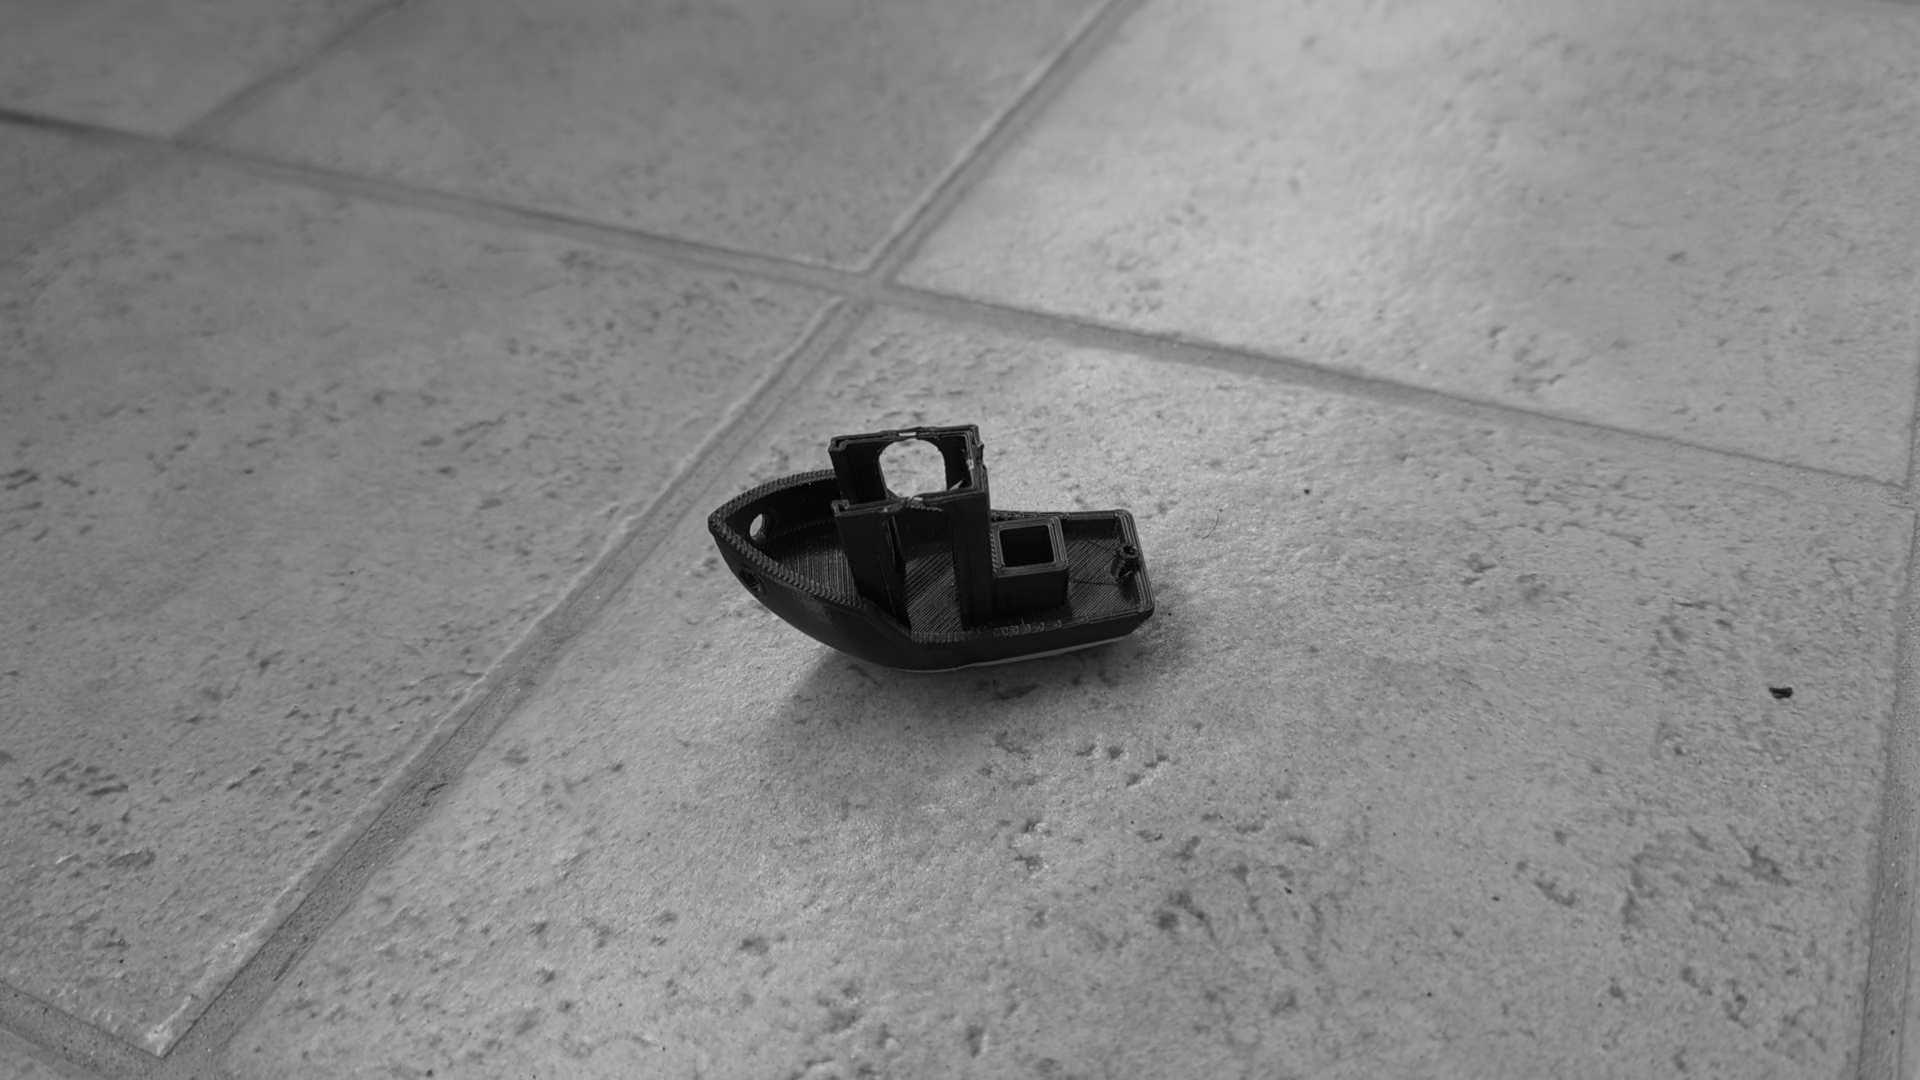
\includegraphics[width=0.7\linewidth]{images/exercise1/videooutimg1}
			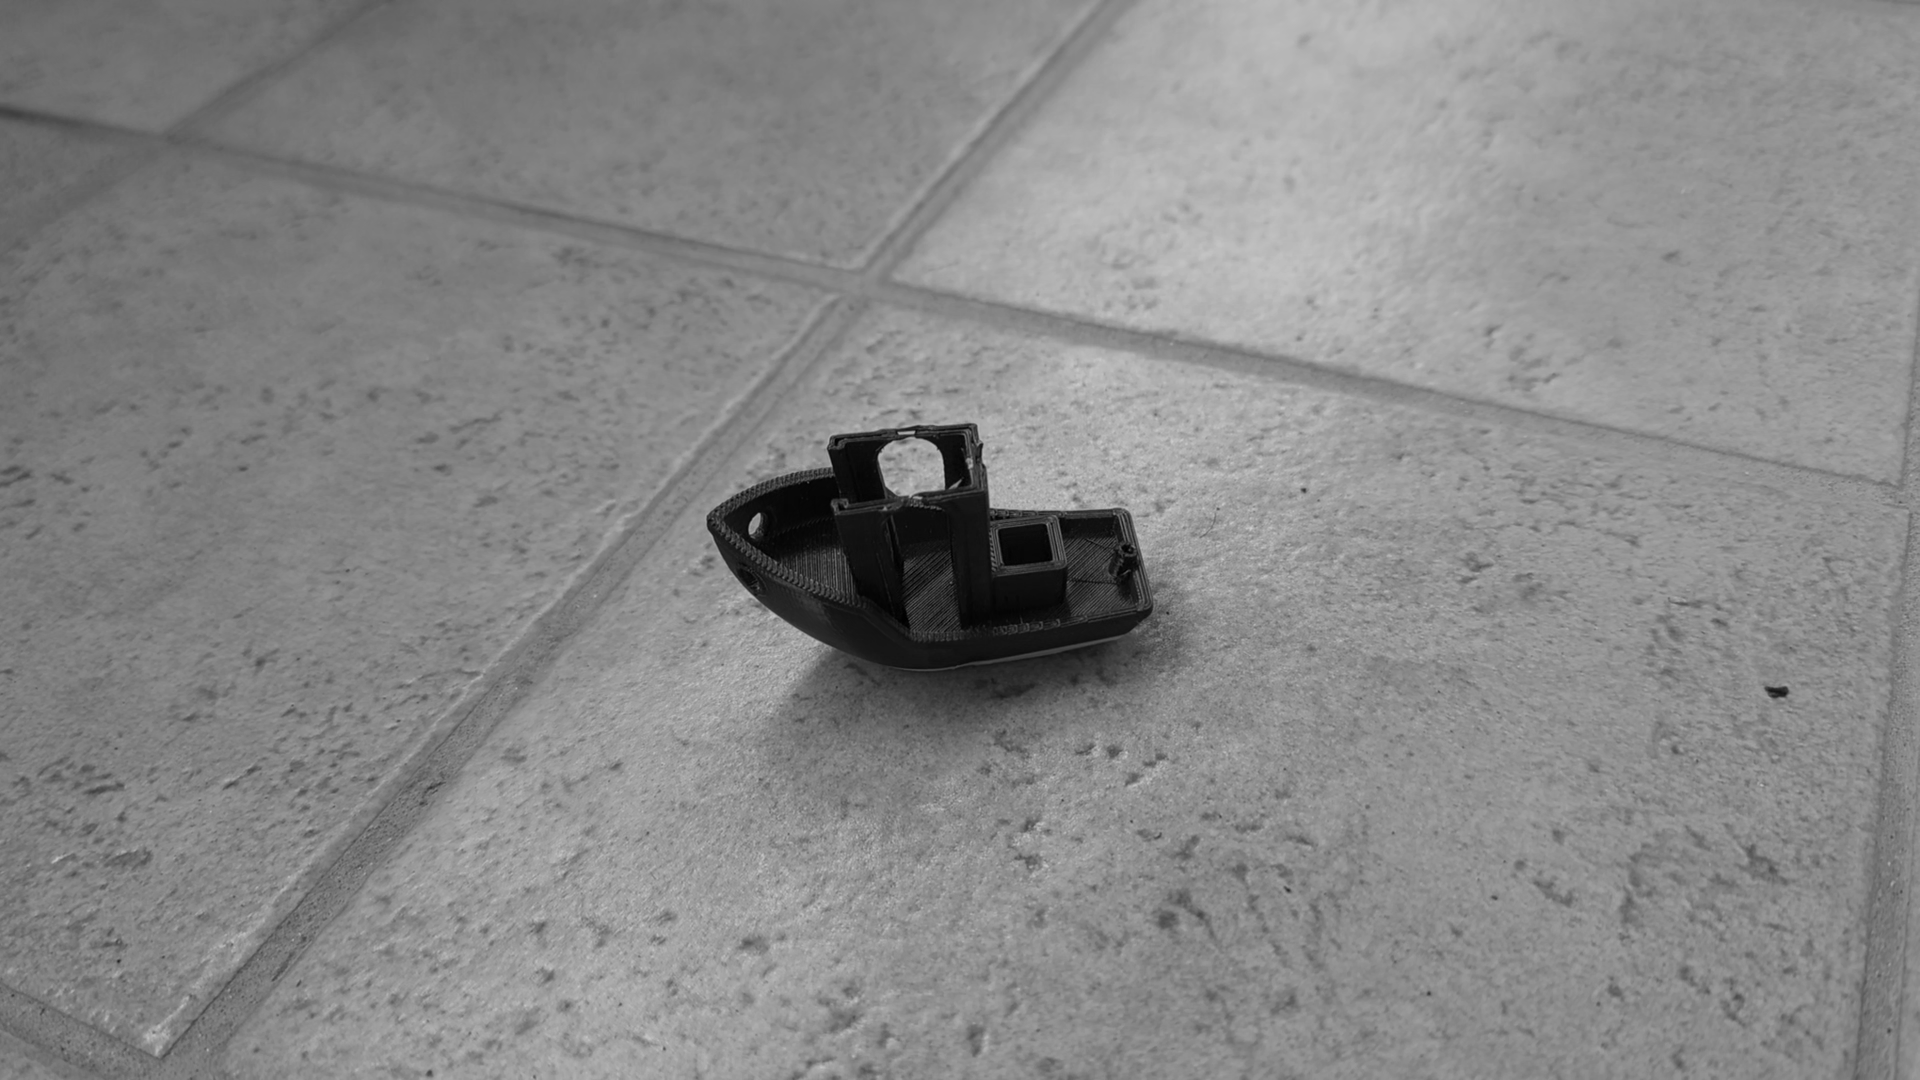
\includegraphics[width=0.7\linewidth]{images/exercise1/videooutimg3}
			\caption{Far input images (11 frames difference).}
			\label{fig:videooutimg3}
		\end{figure}
		And the resulting disparity map.
		\begin{figure}[H]
			\centering
			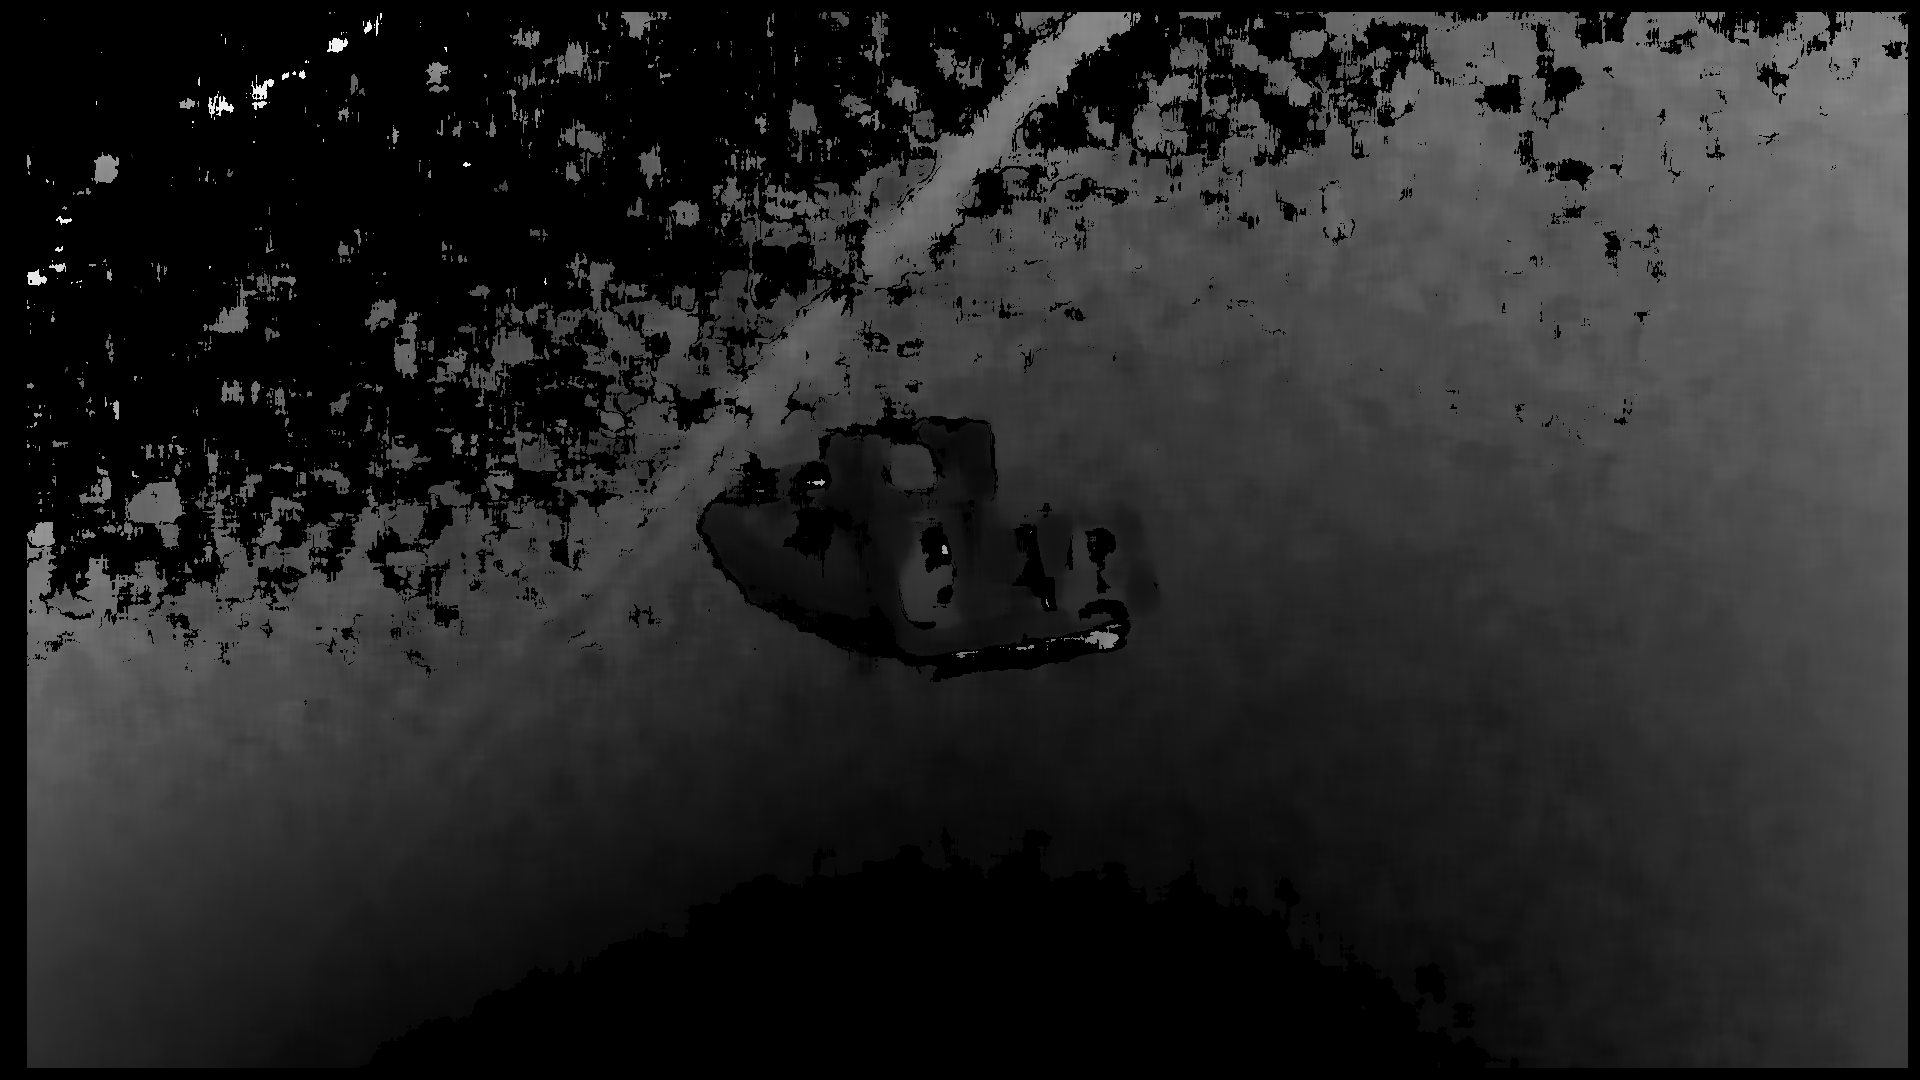
\includegraphics[width=0.7\linewidth]{images/exercise1/videodisparity_far.png}
			\caption{Disparity map using far frames.}
			\label{fig:disparityfar}
		\end{figure}
		
		\item Comment  on  how  the  results  relate  to  the  “distance”  (i.e.  near  vs  far 
		frames) between cameras.
		
		For the sake of it and to better compare the runs I made another video with quicker movements.
		Using the 11th image in that case resulted in a worse disparity map than using just 5 images difference.
		\begin{figure}[H]
			\centering
			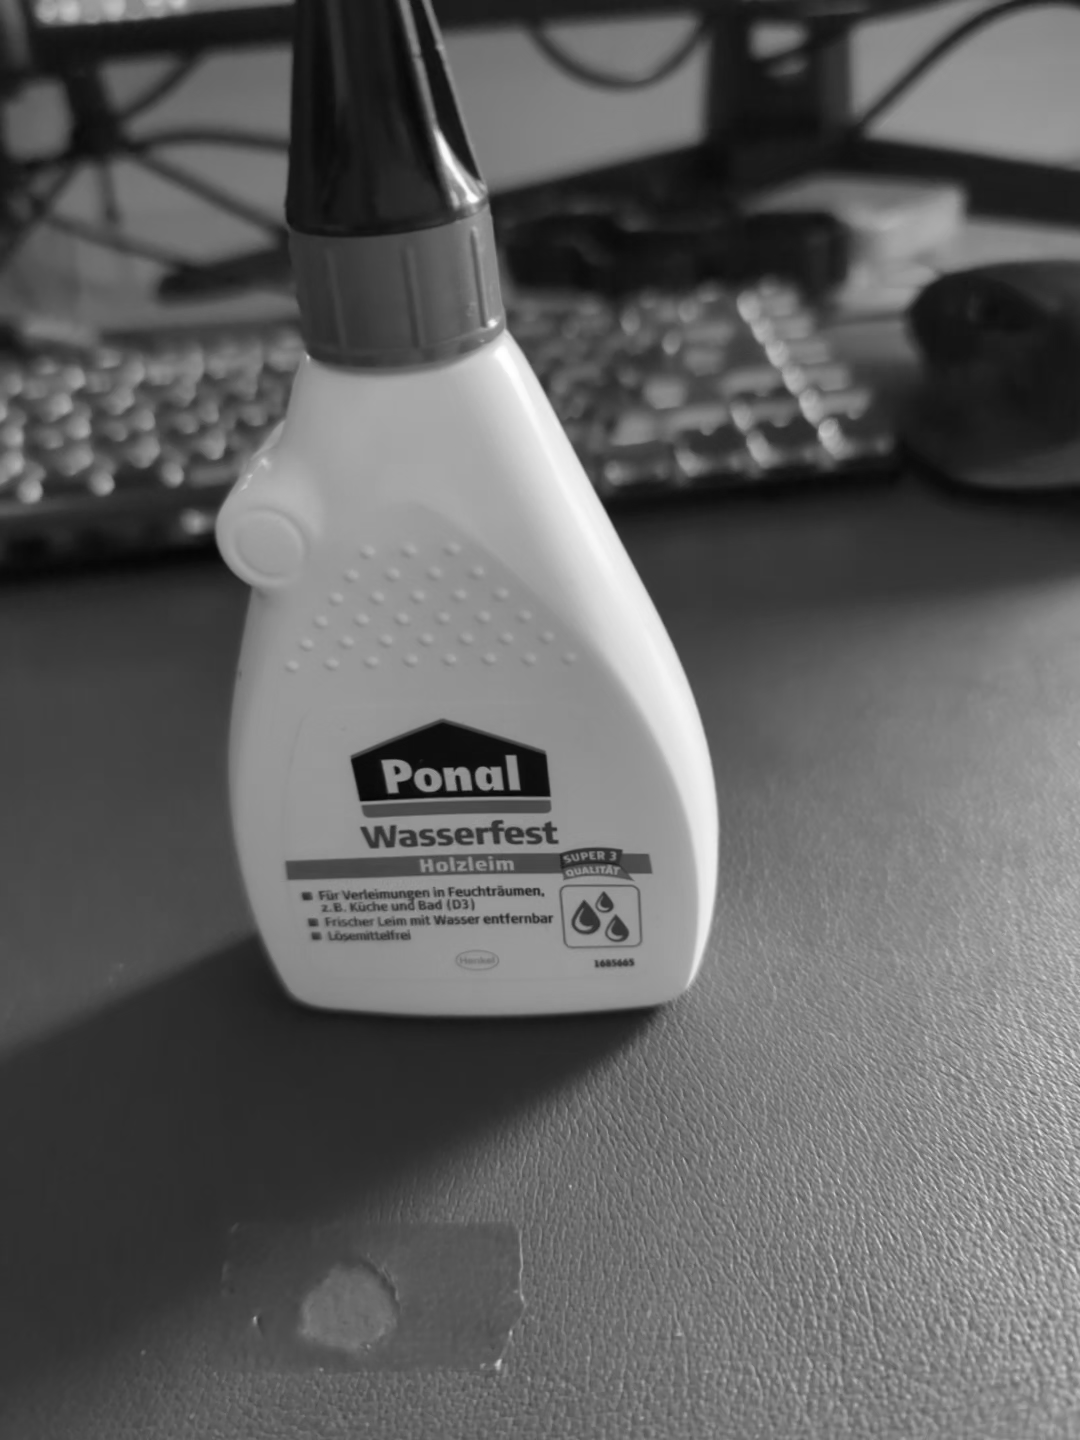
\includegraphics[width=0.3\linewidth]{images/exercise1/glueTestoutimg1.png}
			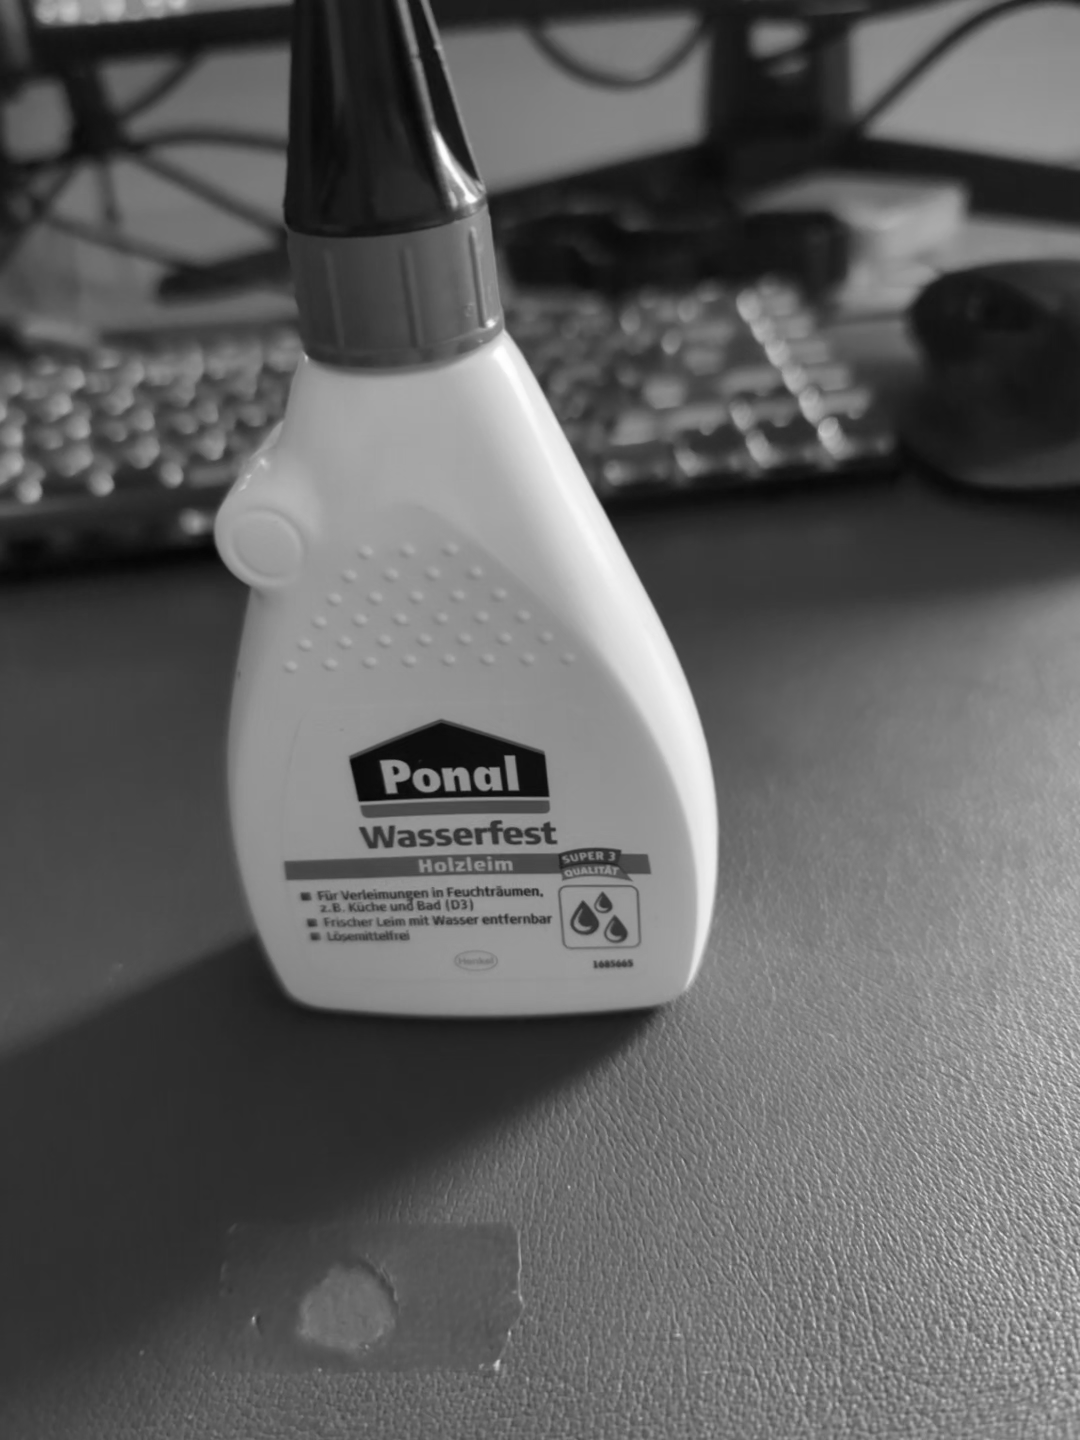
\includegraphics[width=0.3\linewidth]{images/exercise1/glueTestoutimg2.png}
			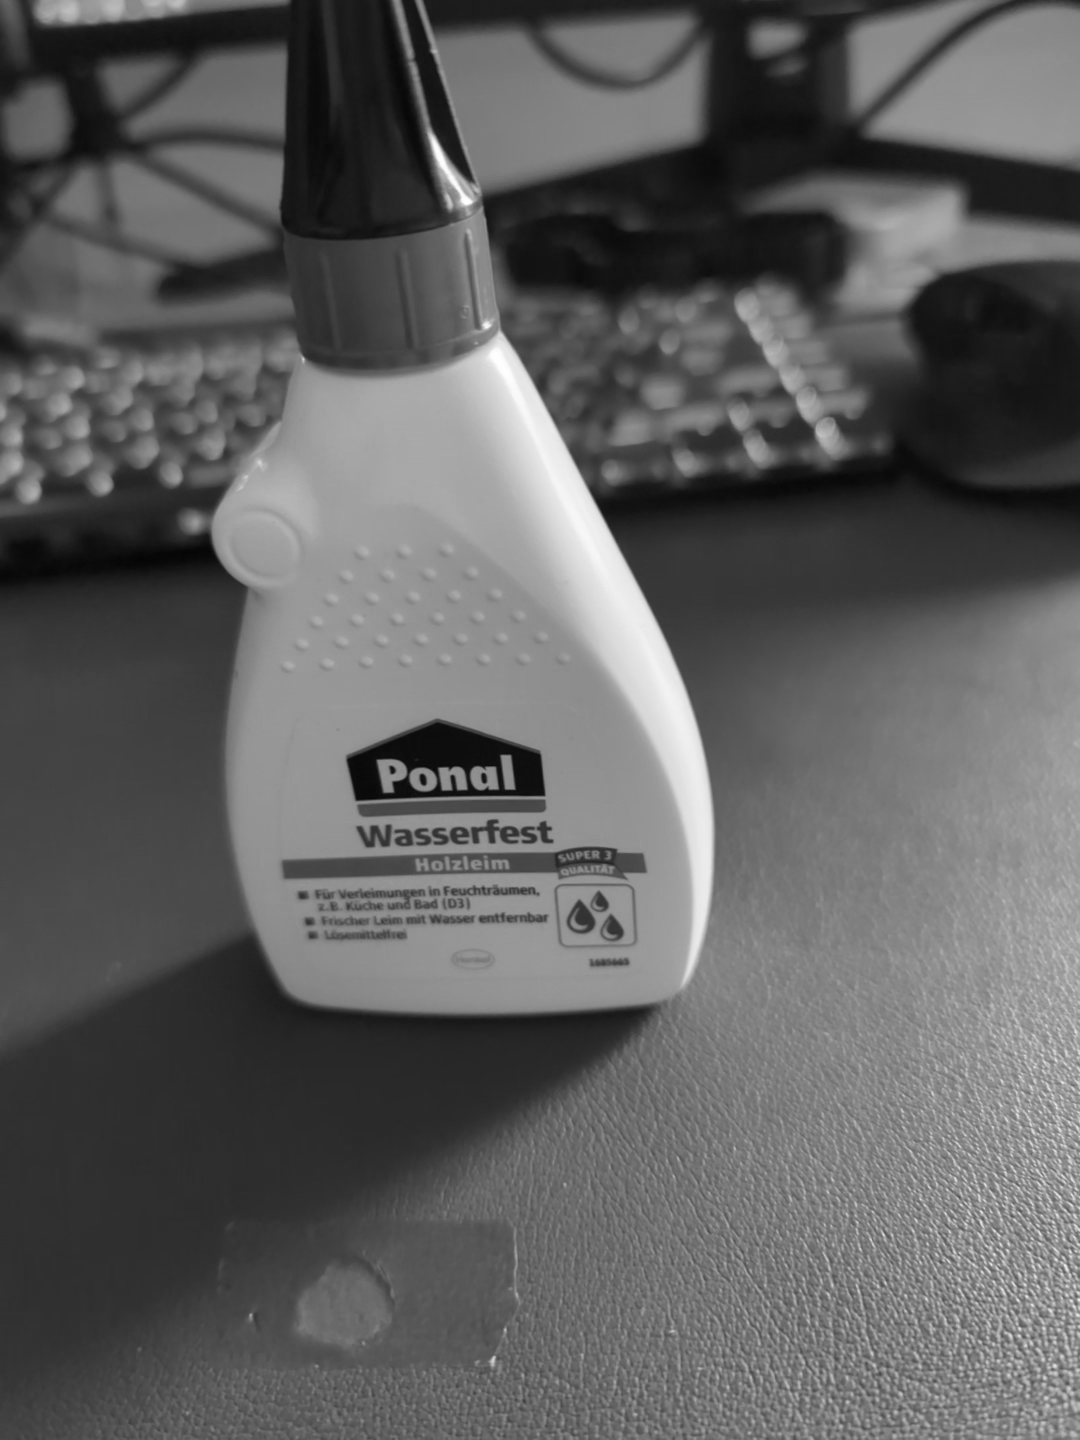
\includegraphics[width=0.3\linewidth]{images/exercise1/glueTestoutimg3.png}
			\caption{Input images}
			\label{fig:disparityglueinput}
		\end{figure}
		\begin{figure}[H]
			\centering
			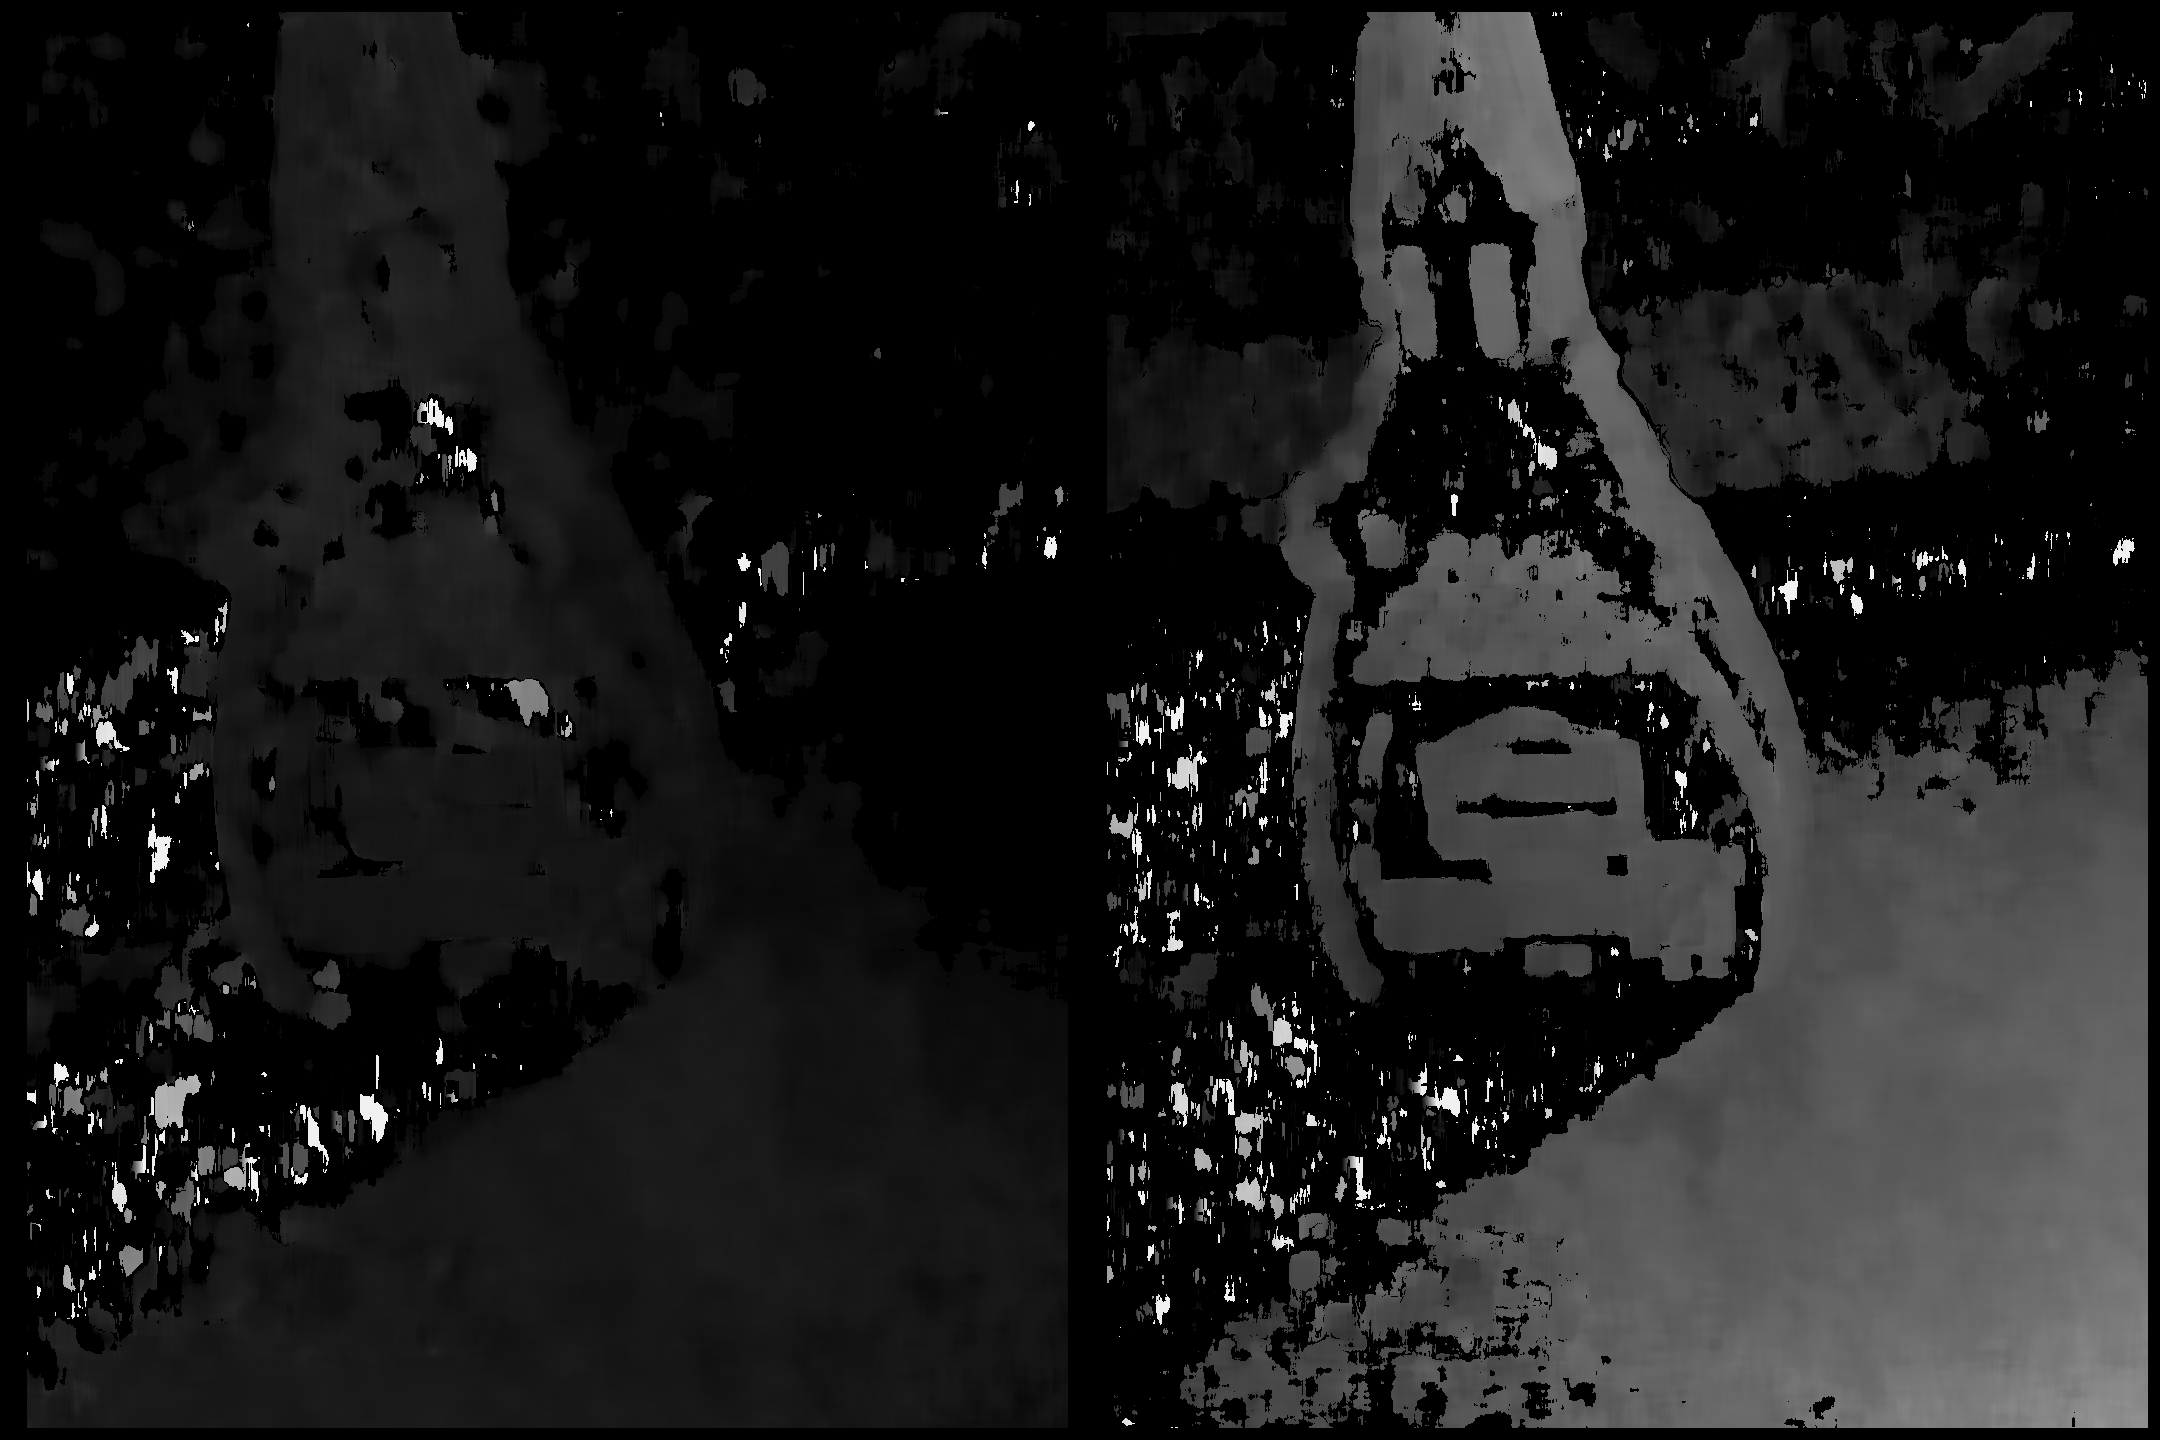
\includegraphics[width=0.8\linewidth]{images/exercise1/glueTestdisparity.png}
			\caption{Disparity map of the near (left) and far (right) images}
			\label{fig:disparityglue}
		\end{figure}
		
		The movement speed has a impact on how many images are ideal for generating the disparity map. Also the surface plays a role as can be seen in the second example where the bottle of glue has a homogenous surface. This is probably the reason why the disparity map has black areas where wide parts are homogenous.
		
		\item Extend the code for stereo rectification.\\
		Note: You can use OpenCV’s cvStereoRectifyUncalibrated() function.
		
		To apply stereo rectification I've used the of the second task.
		The steps that are required are:
		\begin{enumerate}[1.]
			\item Finding key points and their descriptors in both images.
			\item Match the given key points in both images using the descriptors.
			\item After that use the points to find the fundamental matrix of the system.
			\item With the matched points and the fundamental matrix cvStereoRectifyUncalibrated() to get two rectification homography matrices.
			\item (optional) Using these rectification matrices the images can be warped using a OpenCV function to bring the epilines to the same position in both images.
		\end{enumerate}
		\begin{figure}[H]
			\centering
			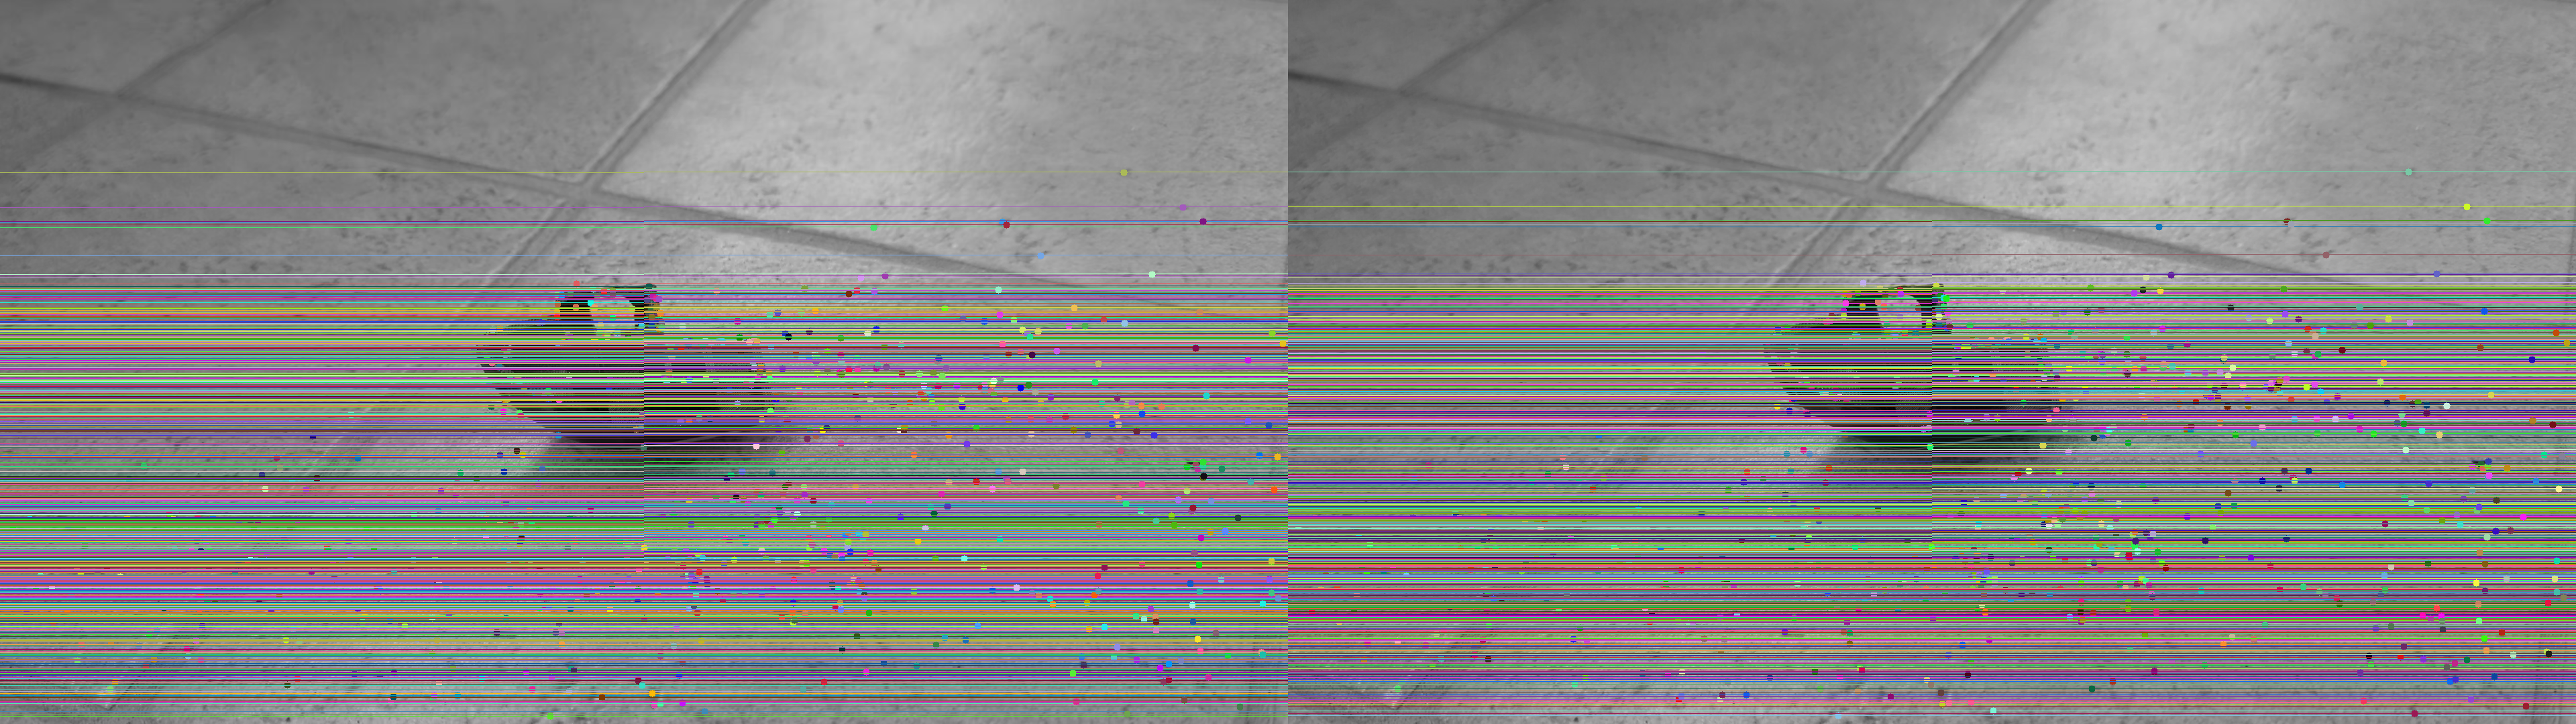
\includegraphics[width=0.7\linewidth]{images/exercise1/videoepilines11skips}
			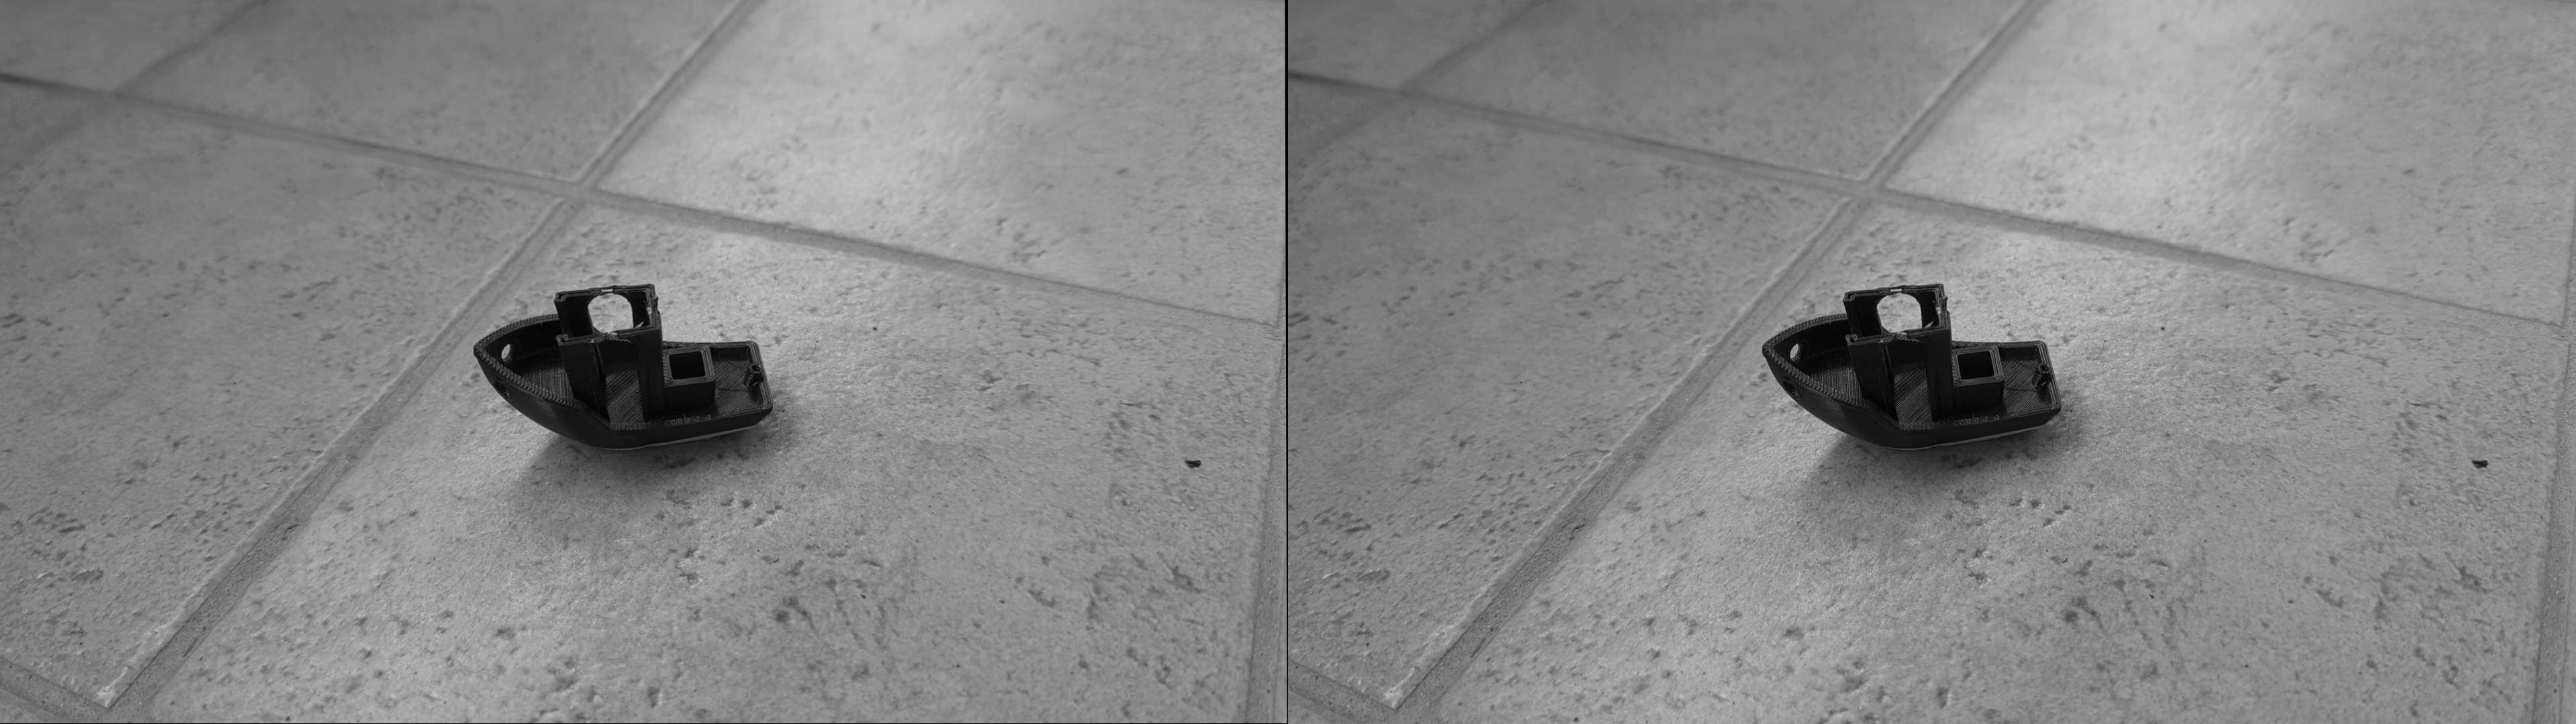
\includegraphics[width=0.7\linewidth]{images/exercise1/videowarped11skips}
			\caption{Epilines in both far frames and below resulting warped frames.}
			\label{fig:videowarped11skips}
		\end{figure}
		
	\begin{figure}[H]
		\centering
		\includegraphics[width=0.7\linewidth]{images/exercise1/videoepilines50skips}
		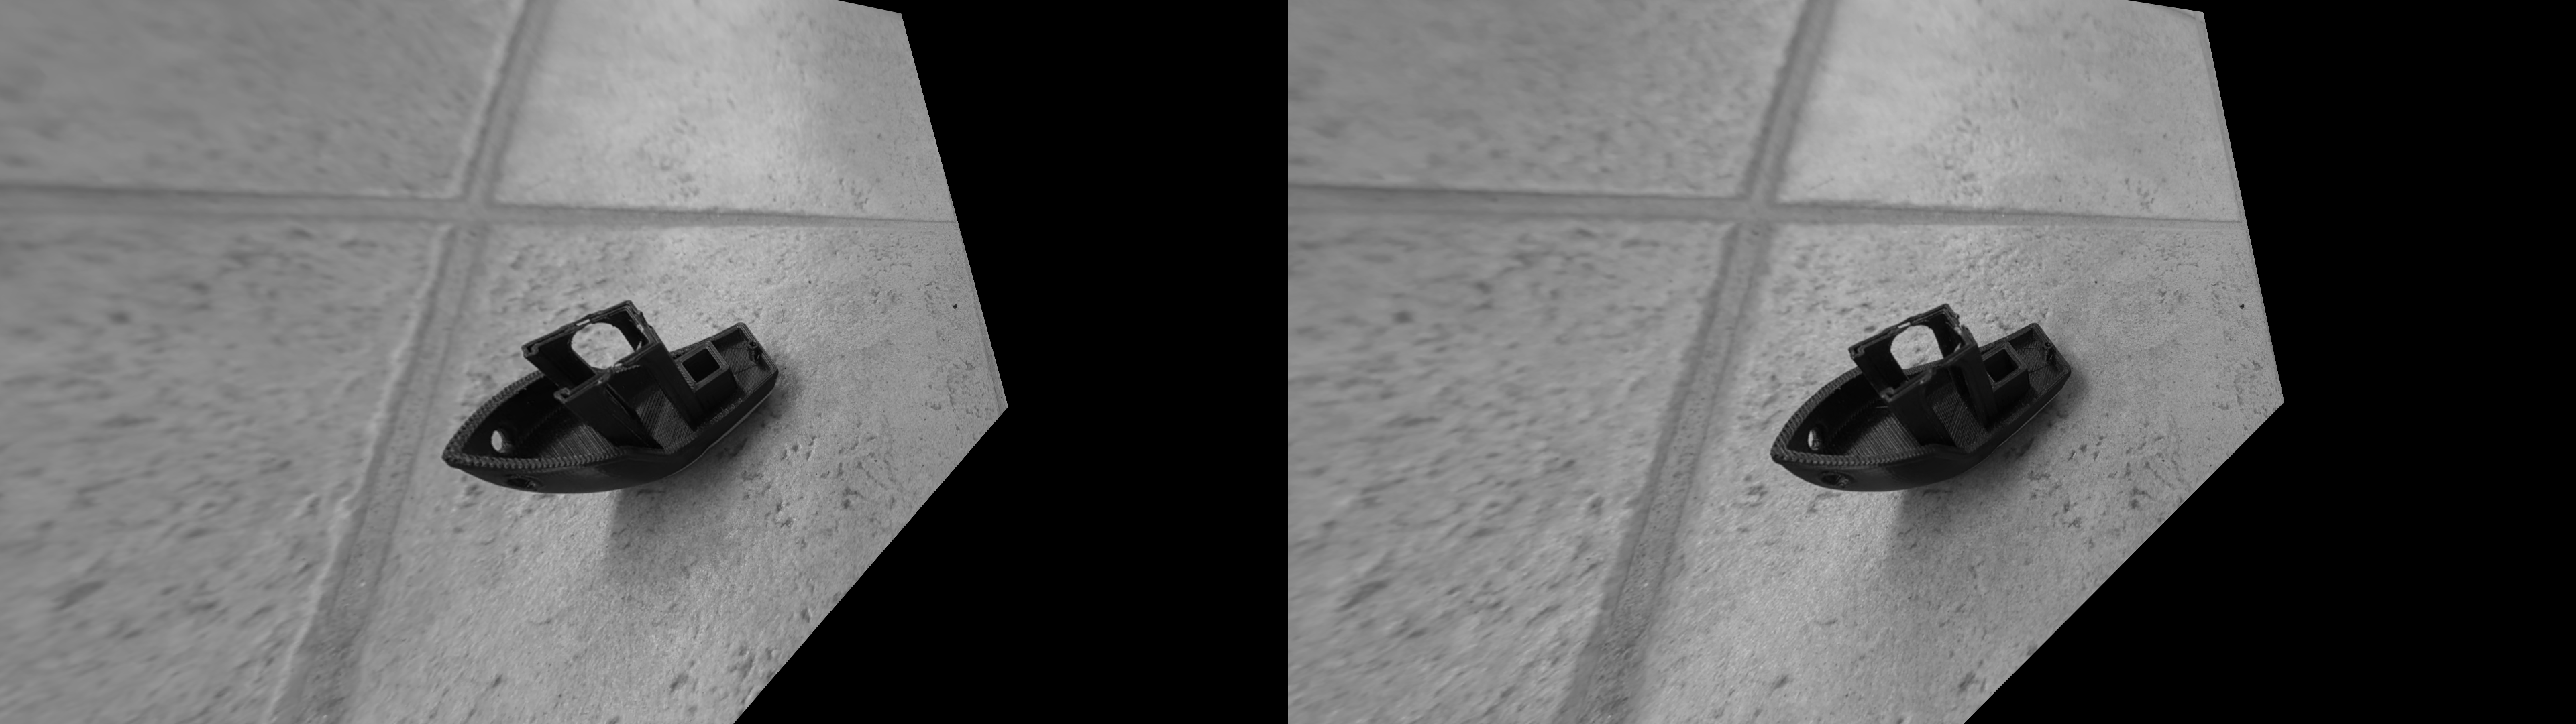
\includegraphics[width=0.7\linewidth]{images/exercise1/videowarped50skips}
		\caption{Epilines in much further (150 images difference) frames and below resulting warped frames.}
		\label{fig:videowarped50skips}
	\end{figure}
	\end{enumerate}
	
	\section*{Task 2}
	(10 points) Work with Epipolar geometry and multi view geometry. Use the 
	frames you generated in the previous exercise:
	\begin{enumerate}[a.]
		\item Analyze  and  test  the  code  from \href{https://docs.opencv.org/4.x/da/de9/tutorial_py_epipolar_geometry.html}{OpenCV Epipolar Geometry Tutorial.}
		\item Change  SIFT  with  two  different  descriptors  of  your  choice  and  compare 
		the results with SIFT.\\\\
		I've decided to use ORB and BRISK as replacements for SIFT as I've worked last semester with SURF and HoG and wanted to check out something new. Also this \href{https://dsp.stackexchange.com/questions/1288/what-are-some-free-alternatives-to-sift-surf-that-can-be-used-in-commercial-app}{signal processing StackExchange Page} helped a bit.
		\begin{figure}[H]
			\centering
			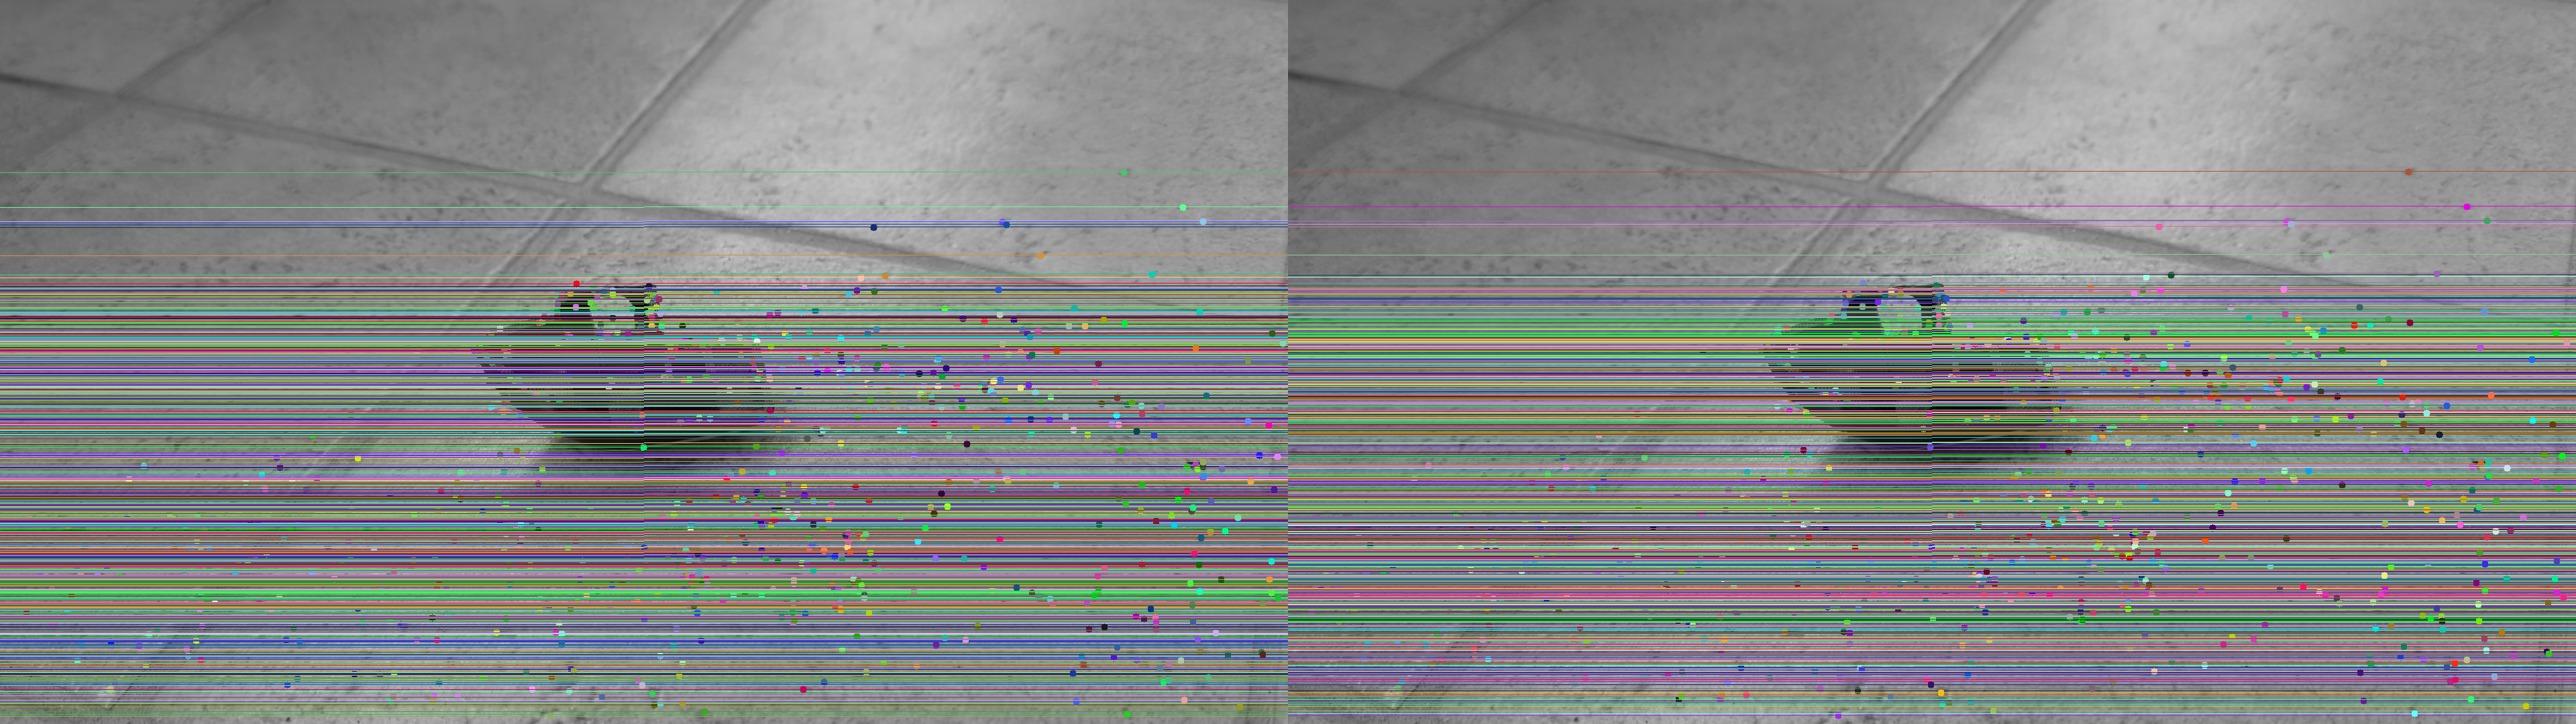
\includegraphics[width=0.7\linewidth]{images/exercise2/exercise1out1ex2_sift_lmeds}
			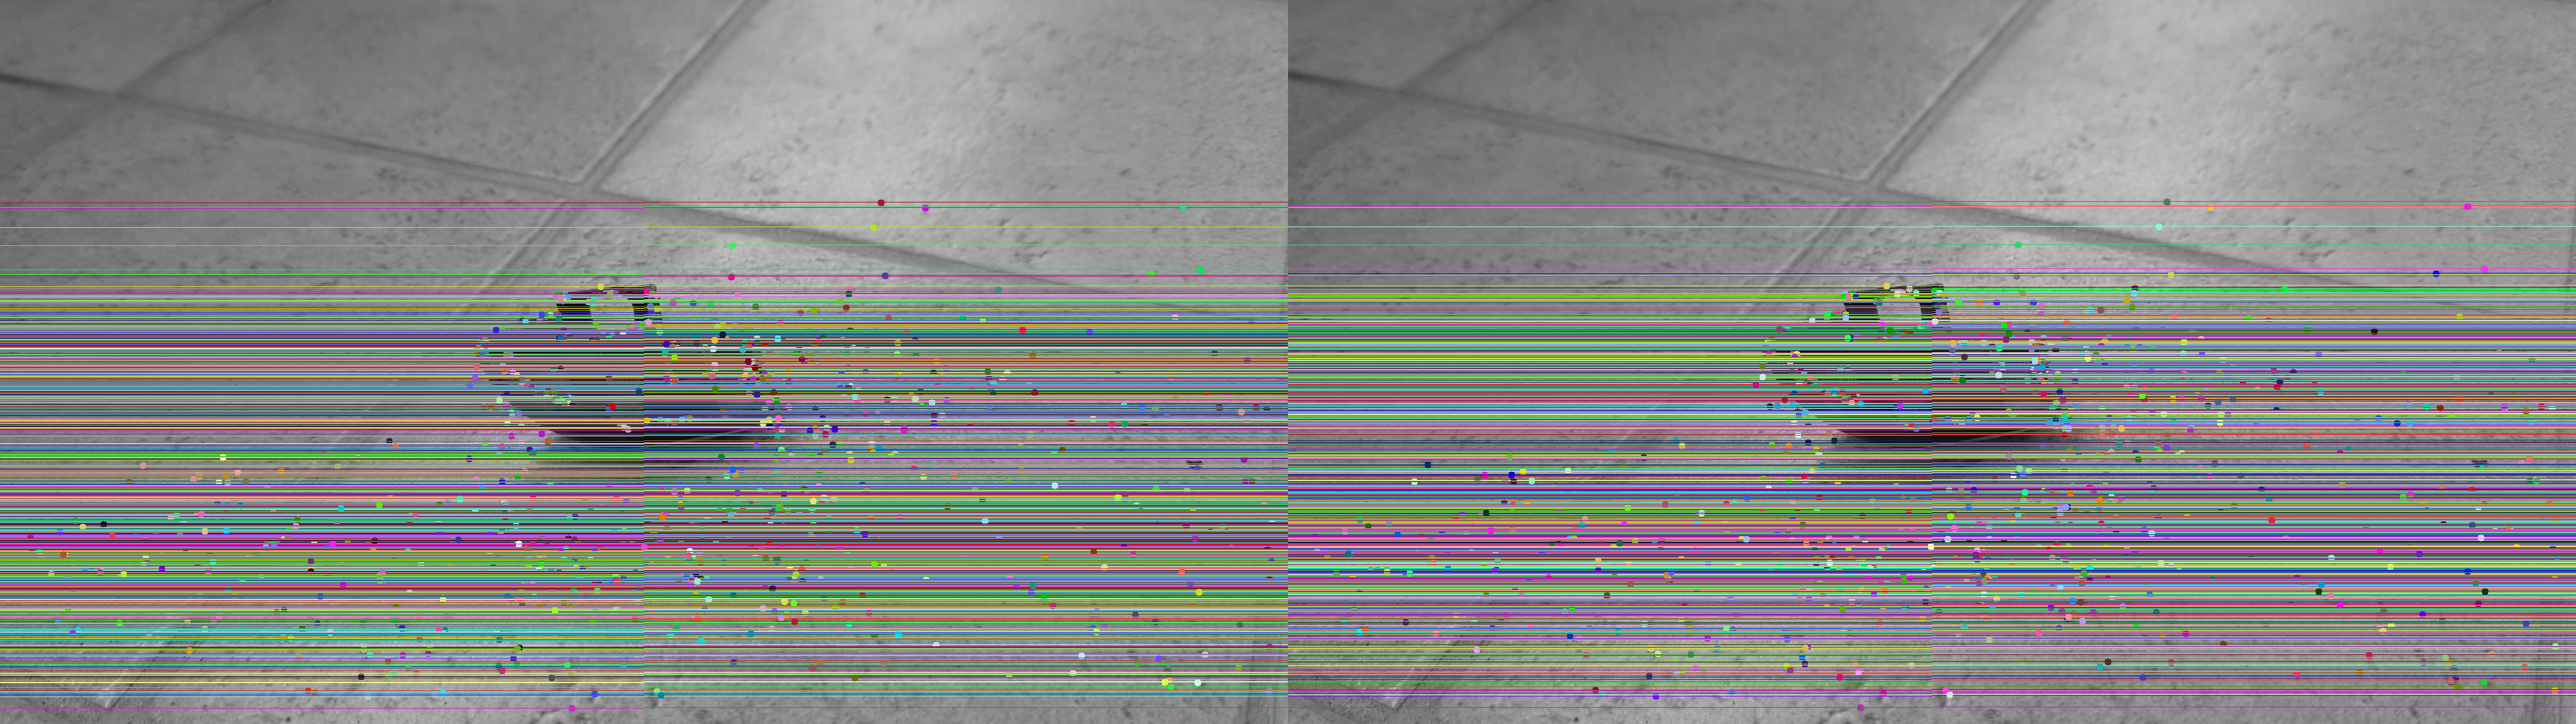
\includegraphics[width=0.7\linewidth]{images/exercise2/exercise1out1ex2_brisk_lmeds}
			\includegraphics[width=0.7\linewidth]{images/exercise2/exercise1out1ex2_orb_lmeds}
			\caption{Output of the execution with SIFT (1), BRISK (2) and ORB (2) using LMEDS.}
			\label{fig:exercise1out1ex2lmeds}
		\end{figure}
		
		Both SIFT and BRISK seem to find good points for LMEDS to work because the lines are parallel, or aligning with to movement of the camera, whilst the epilines calculated with descriptors from ORB seem to be worse.\\
		Between SIFT and BRISK I can't find a great difference, so they are both the "winners".
		
		\item Change  the  computation  of  the  fundamental  matrix  and  compare  the 
		results of RANSAC and LMEDS. What is LMEDS?
		
		LMEDS is short for Least-Median-of-Squares. LMEDS estimates parameters of linear equations with great robustness against outliers.
		It estimates by solving the following non-linear minimization problem:
		\begin{align}
			\text{min } \underset{i}{\text{med }} r^2_i
		\end{align}
		To execute LMEDS there are several steps.
		\begin{enumerate}[1.]
			\item select $n$ random samples from all the datapoints
			\item fit datapoints to a linear (or polynomial) function using a method like least-squares to minimize the distances
			\item before using the above equation, the residual $r$ has to be evaluated
			\item using the residual all points can be evaluated to get their median and save it
			\item repeat the previous steps for $i$ iterations
			\item take the model of the minimal median
		\end{enumerate}
		LMEDS relies on the median as it is much more robust to outliers than using the mean.
		
		
		\begin{figure}[H]
			\centering
			\includegraphics[width=0.7\linewidth]{images/exercise2/exercise1out1ex2_sift_ransac}
			\includegraphics[width=0.7\linewidth]{images/exercise2/exercise1out1ex2_brisk_ransac}
			\includegraphics[width=0.7\linewidth]{images/exercise2/exercise1out1ex2_orb_ransac}
			\caption{Output of the execution with SIFT (1), BRISK (2) and ORB (2) using RANSAC.}
			\label{fig:exercise1out1ex2ransac}
		\end{figure}
		
		Using RANSAC seems to be much more prone to outliers or errors at least in this example. When trying to warp using these epilines just garbage would come out. I guess from these SIFT performed the best but still a lot worse when compared to using LMEDS instead of RANSAC.
		
		\item Apply  the  best  setup  you  have  so  far  to  different  images  of  your  choice 
		from the PhotoTourism challenge dataset \href{https://www.cs.ubc.ca/research/image-matching-challenge/2021/data/}{Image Matching Challenge 2021.}
		
		\begin{figure}[H]
			\centering
			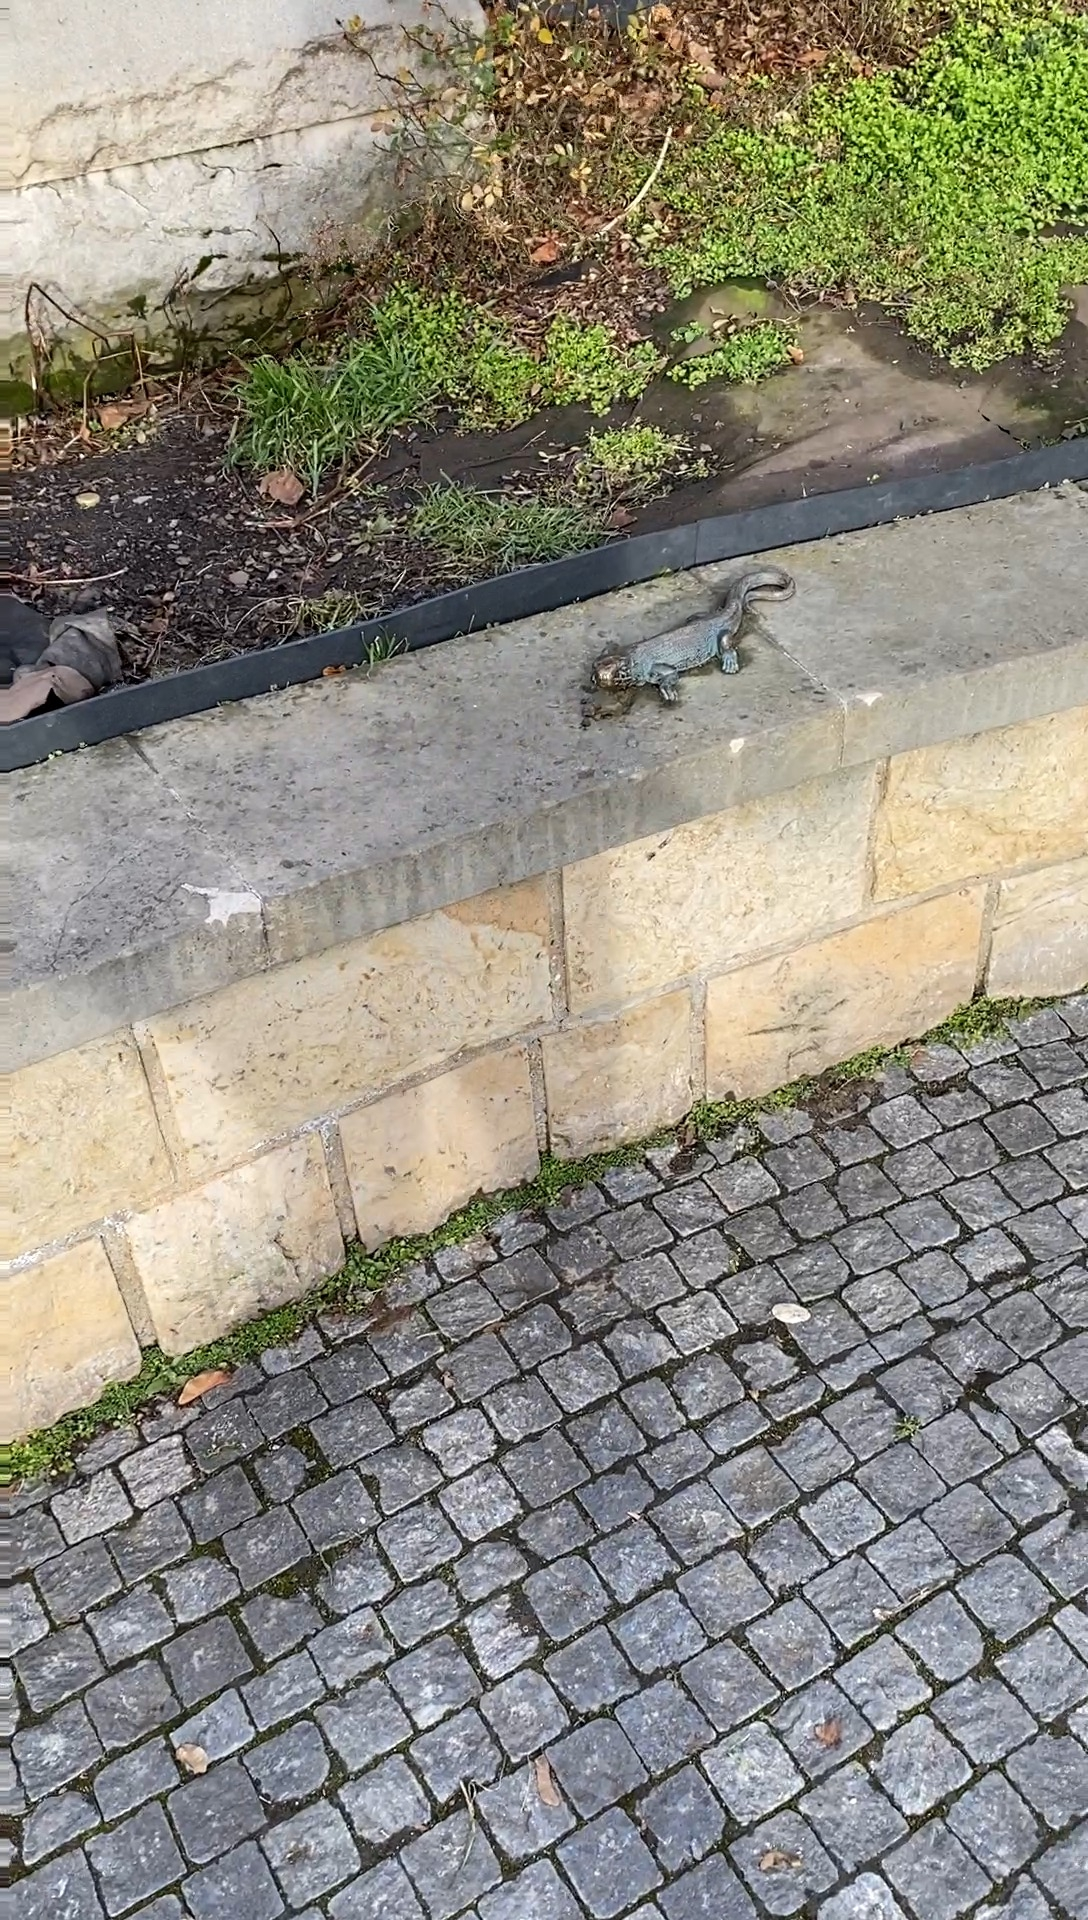
\includegraphics[width=0.45\linewidth]{images/exercise2/frame000071}
			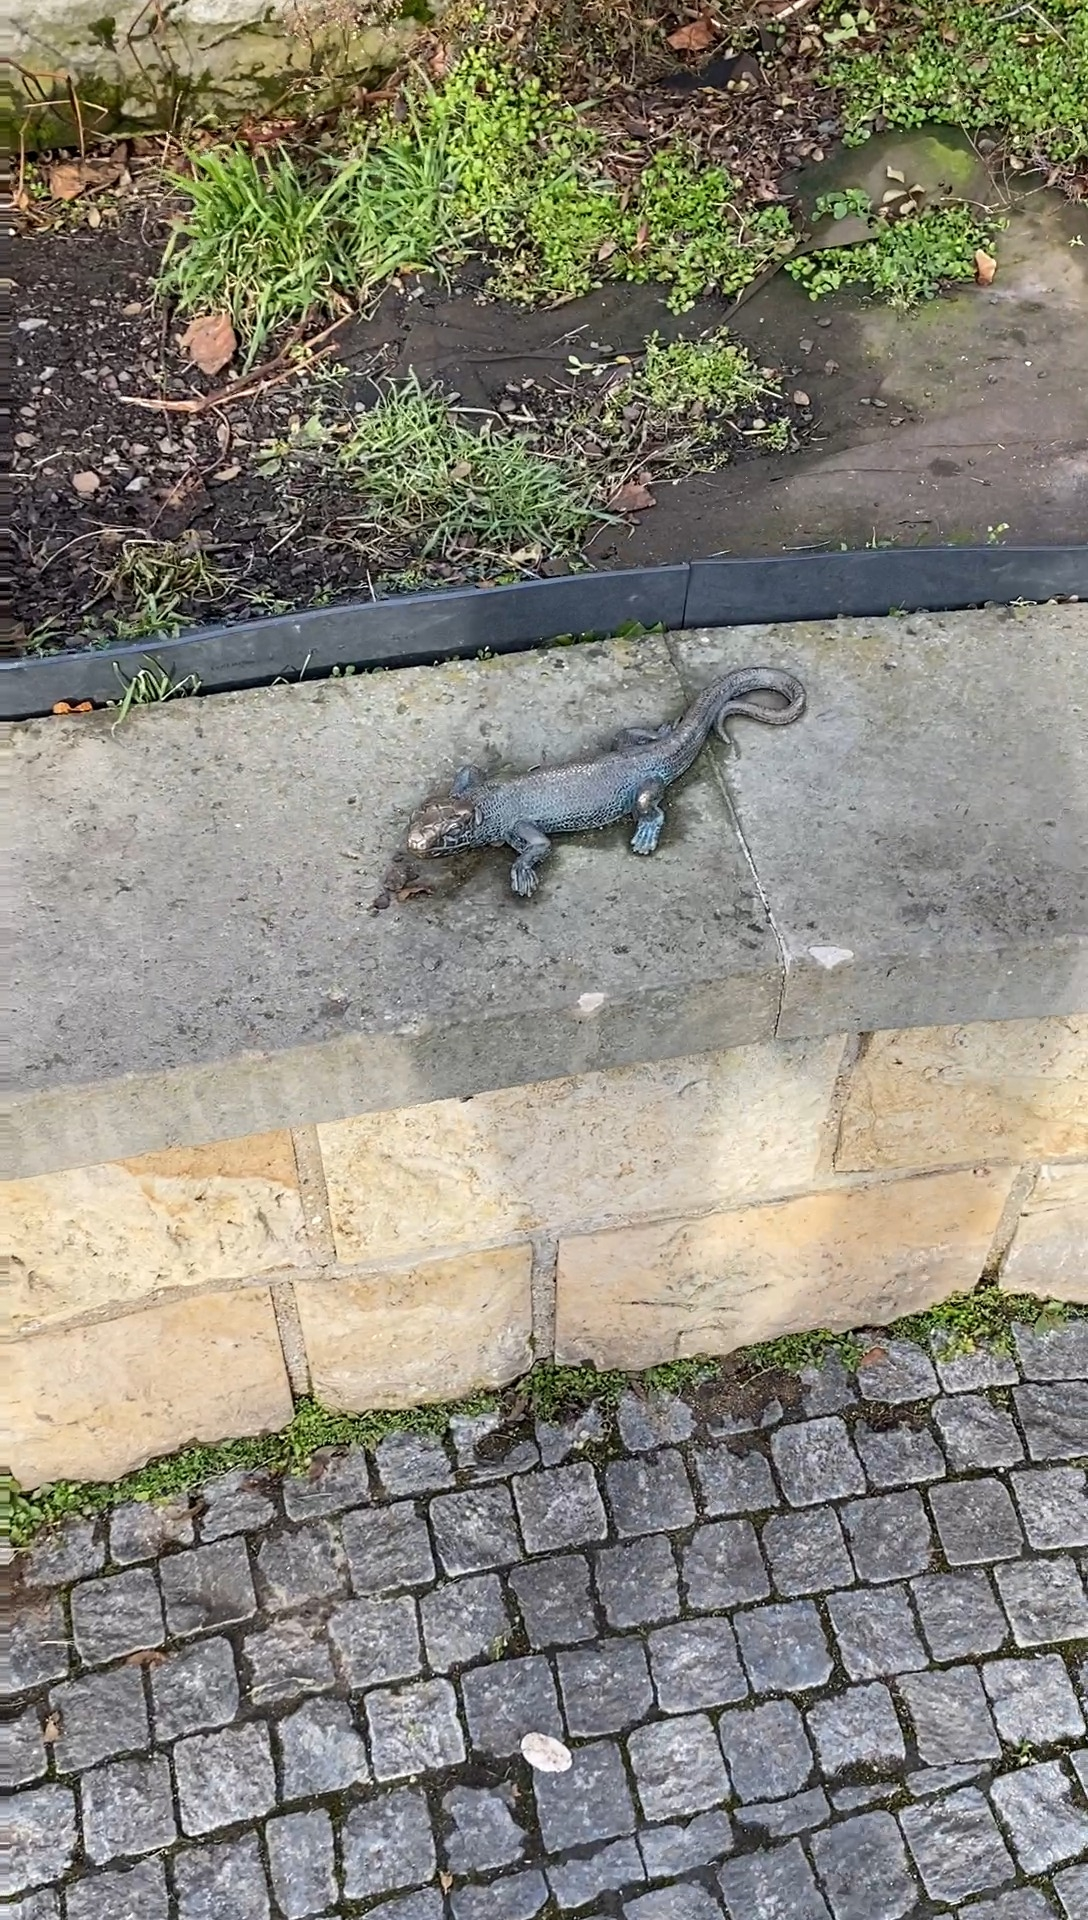
\includegraphics[width=0.45\linewidth]{images/exercise2/frame000075}
			\caption{Samples from the Image Matching Challenge (Prague Parks Lizard).}
			\label{fig:inputlizard}
		\end{figure}
		
		\begin{figure}[H]
			\centering
			\includegraphics[width=0.7\linewidth]{images/exercise2/frame000071.jpgex2_sift_lmeds.png}
			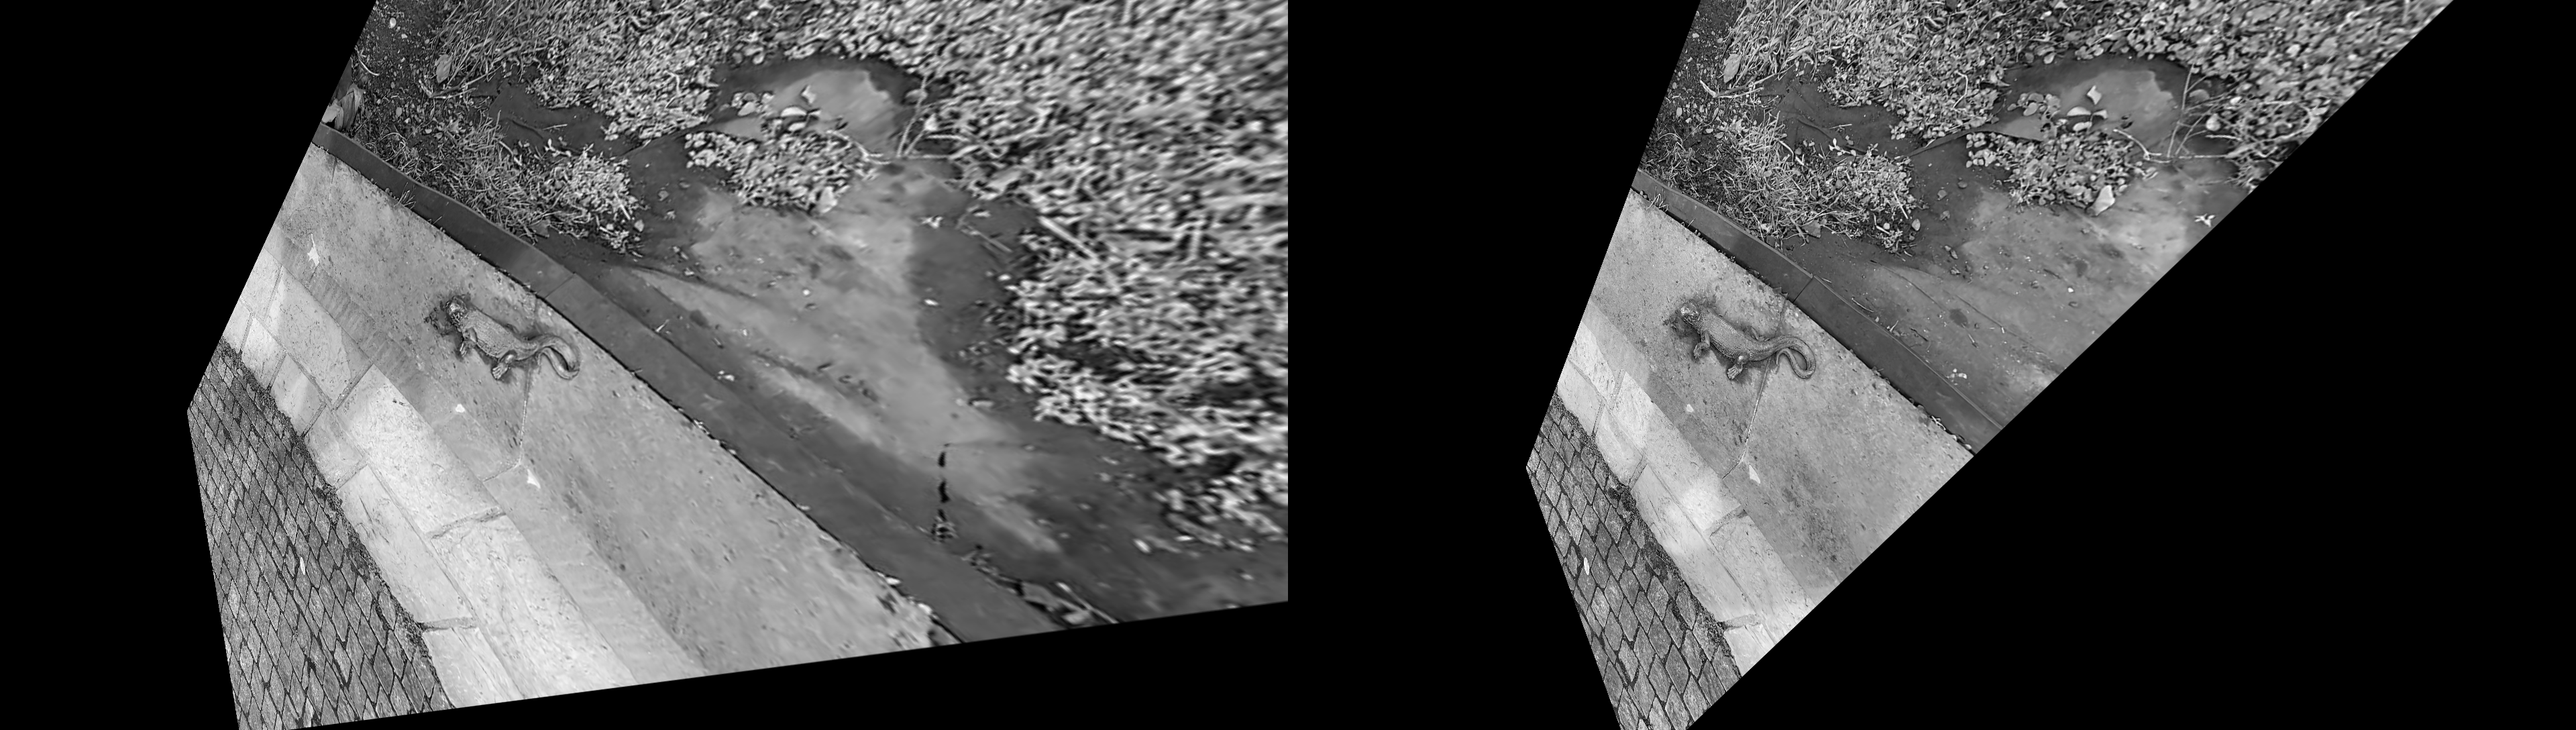
\includegraphics[width=0.7\linewidth]{images/exercise2/frame000071.jpgex2_sift_warped_lmeds.png}
			\caption{Output SIFT/LMEDS combination and warped result.}
			\label{fig:outpChallengeSIFT}
		\end{figure}
		
		\begin{figure}[H]
			\centering
			\includegraphics[width=0.7\linewidth]{images/exercise2/frame000071.jpgex2_brisk_lmeds.png}
			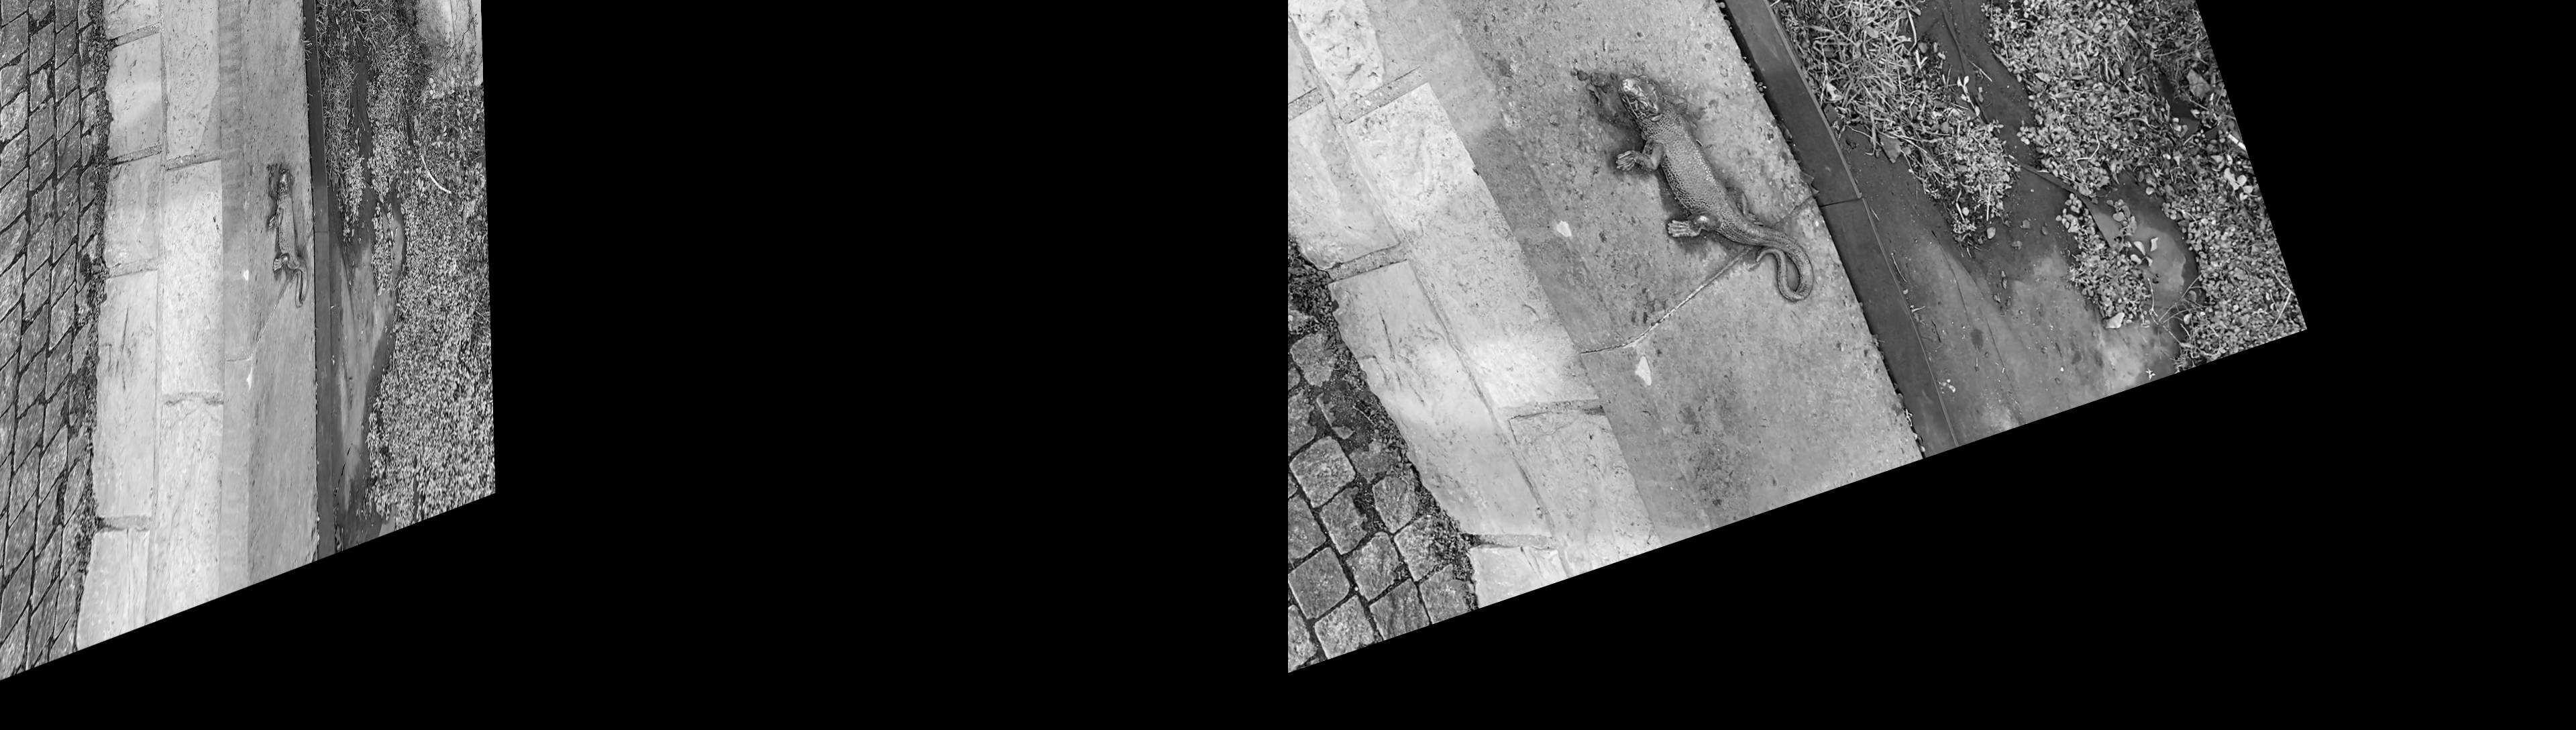
\includegraphics[width=0.7\linewidth]{images/exercise2/frame000071.jpgex2_brisk_warped_lmeds.png}
			\caption{Output BRISK/LMEDS combination and warped result.}
			\label{fig:outpChallengeBRISK}
		\end{figure}
		
		I used both combinations LMEDS with SIFT and BRISK as they performed equally good in the previous exercise. Here in this case SIFT seems to do a better job with the resulting warped image being less squashed together. It would be very interesting if we would use the entire dataset and tried to make a 3D model or reconstruction to see if BRISK/LMEDS would then with more data make a better job or be equally good estimating the epilines compared to SIFT/LMEDS.
		
	\end{enumerate}
\newpage
	\section*{Discussion}
	What  you  learnt  about  this  assignment?  and  how  the  method  can  be 
	improved or extended? What problems did you run into?\\
	I learned how LMEDS works and what it is, and how it compares to RANSAC in a practical manner.
	Also I've deepened my understanding how RANSAC works. And how to use a matcher in this case FLANN to match keypoints in two images.\\
	I played a bit around with the first exercise as I have a OAK-D Lite laying around, this was interesting to see how a (uncalibrated) stereo camera compares to a much simpler approach using just a video.\\\\
	I had just one problem with the first exercise as I didn't know how many frames I would have to use in between to generate a "good" disparity map. I started with a few hundred as the video was recorded with 60 fps but this was too much as the output wasn't any good. To figure this out I just tried a bit around by guessing.
	
	
\end{document}
